\documentclass[a4paper,11pt]{book}
\usepackage{listings}
\usepackage[utf8]{inputenc}
\usepackage[spanish, es-tabla]{babel}

%\usepackage{titlesec}
\usepackage{fancyhdr}
\usepackage[hidelinks]{hyperref}
\usepackage[dvipsnames]{xcolor}
\usepackage{pdfpages}

\usepackage{xspace}

\usepackage{datatool}% http://ctan.org/pkg/datatool
\usepackage{float}
\usepackage{textcomp}


% ********************************************************************
% Información reutilizable
% ********************************************************************
\newcommand{\mySubject}{Trabajo Fin de Grado\xspace}
\newcommand{\myTitle}{Hearcloud\xspace}
\newcommand{\mySubTitle}{Aplicación web orientada a la organización y gestión de música online\xspace}
\newcommand{\mySubTitleENG}{Web application for music management\xspace}
\newcommand{\myDegree}{Grado en Ingeniería Informática\xspace}
\newcommand{\myName}{Mariano Palomo Villafranca\xspace}
\newcommand{\myEmail}{mpvillafranca@correo.ugr.es\xspace}
\newcommand{\myDNI}{20100242J\xspace}
\newcommand{\myProf}{José María Guirao Miras\xspace}
\newcommand{\myFaculty}{Escuela Técnica Superior de Ingenierías Informática y de
Telecomunicación\xspace}
\newcommand{\myFacultyShort}{E.T.S. de Ingenierías Informática y de
Telecomunicación\xspace}
\newcommand{\myDepartment}{Departamento de Lenguajes y Sistemas Informáticos\xspace}
\newcommand{\myUni}{\protect{Universidad de Granada}\xspace}
\newcommand{\myLocation}{Granada\xspace}
\newcommand{\myTime}{\today\xspace}
\newcommand{\myVersion}{Version 0.1\xspace}

% ********************************************************************
% Información de archivo
% ********************************************************************
\hypersetup{
pdfauthor = {\myName (\myEmail)},
pdftitle = {\myTitle},
pdfsubject = {\mySubject},
pdfkeywords = {Hearcloud, aplicación web, música, Django, software libre},
pdfcreator = {LaTeX con el paquete Texmaker},
pdfproducer = {pdflatex}
}

% ********************************************************************
% Estilo de cabeceras
% ********************************************************************
\pagestyle{fancy}
\fancyhf{}
\fancyhead[LO]{\leftmark}
\fancyhead[RE]{\rightmark}
\fancyhead[RO,LE]{\textbf{\thepage}}
\setlength{\headheight}{1.5\headheight}

% ********************************************************************
% Redefinición de comandos
% ********************************************************************
\renewcommand{\chaptermark}[1]{\markboth{\textbf{#1}}{}}
\renewcommand{\sectionmark}[1]{\markright{\textbf{\thesection. #1}}}

% ********************************************************************
% Definición de colores
% ********************************************************************
\definecolor{gray97}{gray}{.97}
\definecolor{gray75}{gray}{.75}
\definecolor{gray45}{gray}{.45}
\definecolor{gray30}{gray}{.94}

% ********************************************************************
% Listados
% ********************************************************************
\lstset{
	aboveskip=0.5cm,
	backgroundcolor=\color{gray97},
	basicstyle=\scriptsize\ttfamily,
	breaklines=true,
	commentstyle=\color{gray45},
	frame=Ltb,
	framerule=0.5pt,
	framesep=0pt,
	framexbottommargin=3pt,
	framexleftmargin=0.1cm,
	framextopmargin=3pt,
	keywordstyle=\bfseries,
	numberfirstline = false,
	numbers=left,
	numbersep=6pt,
	numberstyle=\tiny,
	rulesep=.4pt,
	rulesepcolor=\color{black},
	showstringspaces = false,
	stringstyle=\ttfamily,
	literate={á}{{\'a}}1
	         {é}{{\'e}}1
	         {í}{{\'i}}1
	         {ó}{{\'o}}1
	         {ú}{{\'u}}1
	         {ñ}{{\~n}}1
}
 
% Minimizar fragmentado de listados
\lstnewenvironment{listing}[1][]
	{\lstset{#1}\pagebreak[0]}{\pagebreak[0]}

% ********************************************************************
% Estilo de listados de código
% ********************************************************************
\definecolor{mygreen}{rgb}{0,0.6,0}
\definecolor{mygray}{rgb}{0.5,0.5,0.5}
\definecolor{mymauve}{rgb}{0.58,0,0.82}

\lstset{ %
  backgroundcolor=\color{white},   % choose the background color
  basicstyle=\footnotesize,        % size of fonts used for the code
  breaklines=true,                 % automatic line breaking only at whitespace
  captionpos=b,                    % sets the caption-position to bottom
  commentstyle=\color{mygreen},    % comment style
  escapeinside={\%*}{*)},          % if you want to add LaTeX within your code
  keywordstyle=\color{blue},       % keyword style
  stringstyle=\color{mymauve},     % string literal style
}


\newcommand{\bigrule}{\titlerule[0.5mm]}


% ********************************************************************
% Para ordenar listas de elementos
% ********************************************************************
\newcommand{\sortitem}[1]{%
  \DTLnewrow{list}% Create a new entry
  \DTLnewdbentry{list}{description}{#1}% Add entry as description
}
\newenvironment{sortedlist}{%
  \DTLifdbexists{list}{\DTLcleardb{list}}{\DTLnewdb{list}}% Create new/discard old list
}{%
  \DTLsort{description}{list}% Sort list
  \begin{itemize}%
    \DTLforeach*{list}{\theDesc=description}{%
      \item \theDesc}% Print each item
  \end{itemize}%
}

% ********************************************************************
% Para que en las páginas en blanco no tengan cabeceras
% ********************************************************************
\makeatletter
\def\clearpage{%
  \ifvmode
    \ifnum \@dbltopnum =\m@ne
      \ifdim \pagetotal <\topskip
        \hbox{}
      \fi
    \fi
  \fi
  \newpage
  \thispagestyle{empty}
  \write\m@ne{}
  \vbox{}
  \penalty -\@Mi
}
\makeatother


% ********************************************************************
% Profundidad de la tabla de contenidos
% ********************************************************************
\setcounter{tocdepth}{4}
\setcounter{secnumdepth}{4}

% ********************************************************************
% Párrafos con letras en lugar de números
% ********************************************************************
\renewcommand\theparagraph{\alph{paragraph}}

% ********************************************************************
% Para añadir texto normal entre las referencias de la bibliografía
% ********************************************************************
\newenvironment{bibcomment}{%
  \item[]%
  \begingroup%
  \par%
  \parshape0%
}{%
  \par%
  \endgroup%
}
% ********************************************************************
% Memoria
% ********************************************************************
\begin{document}
\begin{titlepage}
 
\newlength{\centeroffset}
\setlength{\centeroffset}{-0.5\oddsidemargin}
\addtolength{\centeroffset}{0.5\evensidemargin}

\noindent\hspace*{\centeroffset}\begin{minipage}{\textwidth}

\centering

\includegraphics[width=0.9\textwidth]{../images/logo_ugr.jpg}\\[1.4cm]

\textsc{\Large\mySubject\\[0.2cm]}
\textsc{\myDegree}\\[1cm]

{\Huge\bfseries \myTitle\\}
\noindent\rule[-1ex]{\textwidth}{3pt}\\[3.5ex]
{\large\bfseries \mySubtitle}
\end{minipage}

\vspace{2.5cm}
\noindent\hspace*{\centeroffset}\begin{minipage}{\textwidth}
\centering

\textbf{Autor}\\ {\myName}\\[2.5ex]
\textbf{Tutor}\\ {Prof. Dr. \myProf}\\[2cm]

\includegraphics[width=0.3\textwidth]{../images/etsiit_logo.png}\\[0.1cm]
\textsc{\myFaculty}\\
\textsc{---}\\
\myLocation, \myTime\\

\includegraphics[width=0.3\textwidth]{../images/CC-SA-logo.png}
\end{minipage}
\end{titlepage}



\begin{titlepage}
 
 
\setlength{\centeroffset}{-0.5\oddsidemargin}
\addtolength{\centeroffset}{0.5\evensidemargin}
\thispagestyle{empty}

\noindent\hspace*{\centeroffset}\begin{minipage}{\textwidth}

\centering

\vspace{3.3cm}

% Logo del proyecto

\includegraphics[width=0.5\textwidth]{../images/logo_hearcloud_full.png}

 \vspace{0.5cm}

% Title

{\Huge\bfseries \myTitle\\
}
\noindent\rule[-1ex]{\textwidth}{3pt}\\[3.5ex]
{\large\bfseries \mySubTitle.\\[4cm]}
\end{minipage}

\vspace{2.5cm}
\noindent\hspace*{\centeroffset}\begin{minipage}{\textwidth}
\centering

\textbf{Autor}\\ {\myName}\\[2.5ex]
\textbf{Tutor}\\ {Prof. Dr. \myProf}\\[2cm]

\end{minipage}
\vspace{\stretch{2}}

 
\end{titlepage}




\begin{center}
{\large\bfseries \myTitle. \mySubTitle}\\
\end{center}
\begin{center}
\myName\\
\end{center}

% ********************************************************************
% Resumen (Español)
% ********************************************************************
\section*{Resumen}

\bigskip
\noindent{\textbf{Palabras clave}: \textit{aplicación web}, \textit{cloud}, \textit{música}, \textit{organización}, \textit{servidor}, \textit{cliente} }\\

Se pretende desarrollar una \textit{aplicación web} que permita el almacenamiento de ficheros de \textit{música} teniéndolos disponibles en cualquier momento y lugar que se desee, facilitando su accesibilidad a modo de plataforma de computación en la nube (\textit{cloud}). Como resultado, tendremos una herramienta útil y sencilla orientada a la organización de la biblioteca musical del usuario, que podrá realizar modificaciones sobre los metadatos de sus ficheros, tales como ``título'', ``artista'' o ``portada'' y descargarlos de nuevo al sistema local, si quiere, tras los cambios realizados.

El proyecto estará basado en su totalidad en el \textit{software libre}, pudiendo ser adaptado sin dificultad por cualquier otro usuario que así lo quisiera. El desarrollo del servidor se realizará con {\tt Django}, que es un framework para aplicaciones web gratuito y open source, escrito en {\tt Python} que ayuda a desarrollar sitios web más fácil y rápidamente. Haremos uso de {\tt Django template language (DTL)}, que está inspirado en {\tt Jinja2}, para generar archivos HTML basados en \textit{templates}. Por otra parte, en el lado del cliente, utilizaremos código \textit{CSS} para definir y crear la presentación de los documentos HTML con el framework {\tt Twitter Bootstrap} que contiene plantillas de diseño para tipografía, formularios, botones, cuadros, menús de navegación y otros elementos de diseño y nos simplificará la tarea. También se incluirá código \textit{Javascript} y \textit{jQuery} que ayudará a mejorar la experiencia de usuario durante su navegación por el sistema.

Al tratarse de \textit{software libre}, el desarrollo no está limitado al equipo que inicia el trabajo y cualquier usuario puede hacer una contribución al mismo. Para ello, se utilizará un \textit{sistema de control de versiones}, en este caso, {\tt Git}, que es prácticamente un estándar en el mundo. Además, se empleará la plataforma de desarrollo colaborativo (forja) {\tt Github}, que está integrada con Git y nos ayudará en el desarrollo y la distribución del trabajo. De esta forma, cualquier persona que quiera acceder al código del proyecto, podrá hacerlo a través del repositorio y obtener su propia copia gratuita.


\newpage

% ********************************************************************
% Resumen (Inglés)
% ********************************************************************
\begin{center}
{\large\bfseries \myTitle. \mySubTitleENG}\\
\end{center}
\begin{center}
\myName\\
\end{center}

\section*{Abstract}

\bigskip
\noindent{\textbf{Keywords}: \textit{web application}, \textit{cloud}, \textit{music}, \textit{organiation}, \textit{server}, \textit{client} }\\

This project aims to develop a \textit{web application} that lets store \textit{music} files, having them available at every moment and place you want to as a \textit{cloud computing platform}. As a result, we'll have a simple and useful tool oriented to ma}nage the users musical library, who'll be able to edit the files metadatas, like ``title'', ``artist'' or ``cover artwork'' and download them back into their local system, if they want, after those changes.

The development will be \textit{open source}, which means that other users could easily contribute or re-adapt the code if wanted. The server part (backend) will be done with {\tt Django}, a high-level {\tt Python} Web framework that encourages rapid development and clean, pragmatic design. We'll be using {\tt Django template languaje (DTL)}, which is actually based on {\tt Jinja2} syntax, to generate HTML files from templates. Besides that, on the client side (frontend), we'll use \textit{CSS} code to create and define the presentation of that HTML files with the {\tt Twitter Bootstrap} framework, which contains design patterns for fonts, forms, buttons, navegation menus and other elements and will help to make the things easier. Also, we'll include \textit{Javascript} and \textit{jQuery} code to improve the user experience during his navigation across the plattform.

As it's \textit{open source}, the development it's not limited to the team who starts the project so anyone could contribute to it. That's why we'll be using a \textit{version control system}, {\tt Git}, which it's almost an standard all over the world right now. In adition, a web-based Git repository hosting service called {\tt Github} will be used to manage the project work. That way, everyone who want to access the code, could visit the repository link and get his own free copy.

\newpage

% ********************************************************************
% Autorización de publicación en la biblioteca del centro
% ********************************************************************
%\chapter*{}
\thispagestyle{empty}
\noindent\rule[-1ex]{\textwidth}{2pt}\\[4.5ex]

Yo, \textbf{\myName}, alumno de la titulación \myDegree{} de la \textbf{\myFaculty}, con DNI \myDNI, autorizo la
ubicación de la siguiente copia de mi Trabajo Fin de Grado en la biblioteca del centro para que pueda ser
consultada por las personas que lo deseen.

\bigskip
Así mismo, dicha copia se publica bajo licencia \textbf{Creative Commons Attribution-ShareAlike 4.0}. Los terminos de la licencia permiten su copia y/o adaptación en cualquier medio o formato, siempre y cuando se reconozca la autoría y se redistribuya con la misma licencia que el original. La presente documentación, en formato {\tt LaTeX}, puede encontrarse en el repositorio de {\tt Github}: \url{https://github.com/mpvillafranca/hearcloud-doc}.

\vspace{6cm}

\noindent Fdo: \myName

\vspace{2cm}

\begin{flushright}
\myLocation a \myTime.
\end{flushright}

\newpage


% ********************************************************************
% Tutor
% ********************************************************************
%\chapter*{}
\thispagestyle{empty}
\noindent\rule[-1ex]{\textwidth}{2pt}\\[4.5ex]

D. \textbf{\myProf}, profesor del \myDepartment de la \myUni.

\vspace{0.5cm}

\textbf{Informan:}

\vspace{0.5cm}

Que el presente trabajo, titulado \textit{\textbf{\myTitle, \mySubTitle}}, ha sido realizado bajo su supervisión por \textbf{\myName}, y autoriza la defensa de dicho trabajo ante el tribunal que corresponda.

\vspace{0.5cm}

Y para que conste, expiden y firman el presente informe en \myLocation a \myTime.

\vspace{1cm}

\textbf{El tutor:}

\vspace{5cm}

\noindent \textbf{\myProf}

\chapter*{Agradecimientos}
\thispagestyle{empty}

       \vspace{1cm}


Poner aquí agradecimientos...



\tableofcontents
\listoffigures
\listoftables

\mainmatter
\setlength{\parskip}{5pt}

\chapter{Introducción}
\label{cap:introduccion}

\section{Antecedentes históricos}

En el ámbito de las prácticas culturales y aficiones personales de cualquier sociedad, está muy asentado el gusto por la música, sea del tipo que sea, hecho por el cual resulta inevitable que, con el tiempo, hayan surgido dispositivos que permitieran registrar dichos sonidos y almacenarlos para su posterior reproducción.

La historia contemporánea del registro del sonido comienza en 1857, con el fonoautógrafo de Leon Scott, aunque en 1877, Thomas Edison crea el primer artefacto capaz de grabar y reproducir sonido, el fonógrafo, que rápidamente fue sustituido por el gamófono, debido a sus diversas ventajas con respecto a su predecesor. Más tarde, en 1940, aparece el disco de vinilo, logrando una mayor duración y calidad de sonido. Durante ese mismo año, se desarrolla el magnetófono de bobina abierta, que aporta grabaciones de larga duración y buena fidelidad, hecho por el cual tuvo un gran éxito tanto en uso hogareño como profesional. El casete compacto surge posteriormente basándose en esos mismos principios, seguido del microcasete, minicasete, VHS, Casete Compacto Digital y mini DV. Ya en 1979, se produce uno de los inventos más revolucionarios, el disco compacto, que supuso el primer formato digital para audio, desplazando al disco de vinilo y casete. No obstante, el invento más revolucionario en este ámbito, el formato MP3, se empieza a gestar en 1986 y, en 1995 Brandenburg lo utiliza por primera vez en su propio ordenador, convirtiéndose hoy en día en el formato más popular de audio.

Cada soporte de los aquí descritos, ha llevado consigo una forma diferente de organizar los contenidos musicales por parte de los usuarios, tendiendo a una reducción y optimización del espacio necesario para albergar dicha biblioteca musical. 

Con la introducción en el mercado de los ordenadores personales y los diferentes formatos de archivos de audio digital, las alternativas disponibles para llevar a cabo esta organización han aumentado de manera exponencial y se han visto potenciadas, posteriormente, por la aparición de internet.

\section{Motivación}

Uno de los principales problemas que surgen del almacenamiento de música en los ordenadores personales en la actualidad es su portabilidad, pues existe un gran abanico de posibilidades en cuanto a dispositivos de reproducción se refiere: reproductores MP3, iPods, teléfonos móviles, tabletas, automóviles, etc. 

No obstante, normalmente, el usuario debe elegir un dispositivo en el que almacenar su biblioteca y, si quisiera portarla a otro, copiarla al mismo mediante algún método de transferencia de ficheros. El principal problema de ello, es mantener la sincronización entre estos dispositivos.

Este proyecto surge como respuesta a esa necesidad de los usuarios de organizar su música y mantenerla ``sincronizada'' en todos sus dispositivos, de manera que esté disponible en lugar que se desee.



\chapter{Objetivos}
\label{cap:objetivos}

El objetivo del proyecto es la creación de una plataforma web donde los usuarios puedan almacenar su biblioteca musical y ésta se encuentre disponible para ellos en cualquier lugar y momento que deseen a través de internet. Se pretende establecer una metodología de trabajo flexible, en la que puedan ir incluyéndose mejoras incrementalmente manteniéndose la integridad del sistema. \\

Si bien, éste es el objetivo final a alcanzar, podemos destacar una serie de objetivos principales a cumplir que darán pié al mismo:

\begin{itemize}
	\item \textbf{OBJ-1.} Estudiar el estado actual del mercado en cuanto a productos y soluciones de este tipo, analizando sus ventajas y desventajas correspondientes.

	\item \textbf{OBJ-2.} Proporcionar una metodología flexible y sencilla, pero a la vez robusta y viable que se pueda aplicar durante el desarrollo íntegro del proyecto. 

	\item \textbf{OBJ-3.} Crear un sistema flexible que pueda ser adaptado con facilidad por otros usuarios que así lo deseen, ya sea como contribución al proyecto original o para su propia implantación de manera externa.

	\item \textbf{OBJ-4.} Dotar al proyecto de la posibilidad de ser alojado en la nube, buscando una alta disponibilidad y calidad en la experiencia de usuario.

	\item \textbf{OBJ-5.} Llevar a cabo un desarrollo abierto tanto del proyecto como de su documentación (véase apéndice \hyperref[sec:licencias]{Licencias}), dando como resultado un producto \textit{open source} basado en tecnología libre.
\end{itemize}

\bigskip

\section{Alcance de los objetivos}

La plataforma resultante podrá ser implantada en cualquier servidor en el que quiera desplegarse siempre que puedan satisfacerse las dependencias necesarias. Por otra parte, al tratarse de un sistema \textit{open source} y, puesto que el software es de dominio público, se podría buscar un posible nicho de mercado en la prestación del servicio en la nube.


\chapter{Planificación y análisis}
\label{cap:panificacion-analisis}

\section{Planificación}
\label{sec:planificacion}

Tras definir los objetivos a completar en el transcurso de este proyecto, pasamos a exponer la planificación temporal propuesta, que será dividida en diferentes fases y presentada, finalmente, mediante un diagrama de \textit{Gantt}.

\subsection{Fases}

A continuación se describen cada una de las fases propuestas así como una serie de actividades previstas por cada una de ellas.

\begin{itemize}
	\item \textbf{Fase 1}. Especificación del proyecto. Consiste en establecer los objetivos a cumplir para completar el proyecto, así como la búsqueda de información necesaria para llevarlo a cabo.
	\begin{itemize}
		\item Búsqueda de información.
		\item Determinación de objetivos.
		\item \underline{\textit{Estimación}}: 20 horas
	\end{itemize}
	
	\item \textbf{Fase 2}. Planificación. Elaboración y desarrollo de la documentación correspondiente a la planificación del proyecto.
	\begin{itemize}
		\item Listar las fases del proyecto.
		\item Especificar las actividades de las que constará cada fase.
		\item Análisis de presupuesto.
		\item Temporización
		\item \underline{\textit{Estimación}}: 20 horas
	\end{itemize}
	
	\item \textbf{Fase 3}. Análisis y diseño. Estudio del problema a abordar, análisis de requisitos y diagramas asociados de cara a concretar la forma en que se desarrollará.
	\begin{itemize}
		\item Análisis de requisitos
		\item Diseño de diagramas
		\item \underline{\textit{Estimación}}: 40 horas
	\end{itemize}
	
	\item \textbf{Fase 4}. Implementación. Tras las fases de planificación y diseño, se pasa a codificar todo lo necesario con el fin de cumplir los \hyperref[cap:objetivos]{objetivos propuestos}.
	\begin{itemize}
		\item Selección de herramientas.
		\item Desarrollo \textit{Backend}: modelos, \textit{urls}, controladores.
		\item Desarrollo \textit{Frontend}: vistas, \textit{templates}, \textit{HTML}, \textit{CSS}, \textit{Javascript}.
		\item Tareas de automatización (\textit{DevOps}).
		\item \underline{\textit{Estimación}}: 160 horas
	\end{itemize}
	
	\item \textbf{Fase 5}. Pruebas. Se hará uso de \textit{tests unitarios}, entre otros procedimientos, para probar el código generado y que el sistema funciona correctamente.
	\begin{itemize}
		\item Pruebas del software: modelos, vistas, formularios.
		\item \underline{\textit{Estimación}}: 35 horas
	\end{itemize}
	
	\item \textbf{Fase 6}. Documentación final. Completar la documentación restante asociada al proyecto, como manuales de usuario o anexos.
	\begin{itemize}
		\item Documentación del sistema.
		\item Manual de usuario.
		\item Documentación del proyecto.
		\item \underline{\textit{Estimación}}: 25 horas
	\end{itemize}
\end{itemize}

\subsection{Recursos humanos}

Además del autor del proyecto, se contempla la participación de representantes del público objetivo destinatario del producto con el fin de recabar información relativa a su utilidad, así como posibles deficiencias, beneficios y/o mejoras.


\subsection{Temporización}

Por último, para poder apreciar de una forma algo más visual la planificación temporal descrita, generamos un diagrama de \textit{Gantt} que represente dicha información.

TODO: AQUÍ DIAGRAMA DE GANTT

\subsection{Presupuesto}

La principal ventaja del uso de software libre es que no es necesario adquirir licencias de pago para usar dicho software. Como las herramientas que se van a utilizar y todo el código que se genere será libre, el coste económico y, por tanto, el presupuesto inicial del proyecto será cero.\\

El único aspecto económico relevante que habrá que considerar en este caso será, entonces, el de los posibles gastos por el uso de un servidor en el que se implante el software.

\section{Análisis}
\label{sec:analisis}

\subsection{Estudio de mercado}

La creación de un producto software nuevo no es una tarea sencilla, sobre todo cuando no cuentas con una mínima información acerca del mercado en el que esperas que se desenvuelva. Por eso, realizar un estudio de las alternativas ya existentes, nos ayudará a obtener datos sobre nuestros ``competidores'' y localizar posibles enfoques promocionales de cara a resaltar las ventajas que nuestra solución pueda ofrecer frente a las suyas. Entre ellos, destacamos:

\subsubsection{Spotify \cite{Spotify}}
Spotify es un servicio de reproducción de música vía streaming que permite escuchar un amplio catálogo en modo radio o bien buscando por artista, álbum o listas de reproducción. Si embargo, éste es ofrecido por la plataforma y no es posible almacenar tu própia música en ella para combinarlo, de alguna manera, con lo que ya ofrecen ellos. Por tanto, si una canción no se encuentra entre sus bases de datos, tendrás que recurrir a otra alternativa para poder oirla. No obstante, si no es el caso, la plataforma representa una gran ventaja para disponer de tu selección musical en la nube y organizada según tus propios criterios en modo de listas de reproducción.\\

El servicio puede utilizarse de dos formas diferentes: la versión gratuita, con la publicidad ocasional mencionada y la limitación de no poder escuchar canciones bajo demanda en la versión móvil, y la versión ``\textit{premium}'', que elimina todas estas limitaciones, ofrece una calidad de audio mejor y la posibilidad de descargar la música para escucharla en modo sin conexión.

\subsubsection{Soundcloud \cite{Soundcloud}}
Soundcloud es una plataforma de distribución de audio en línea que permite a sus usuarios subir, grabar, promocionar y compartir su música de autoría original. Está, por tanto, orientada sobre todo a músicos y sellos discográficos, aunque cualquier usuario registrado tiene acceso a la música de estos y puede almacenarla en listas de reproducción, públicas o privadas, en su propio perfil para su reproducción.\\

La plataforma ofrece servicios premium en dos modalidades diferentes: ``\textit{Pro}'', que permite subir hasta seis horas de audio y, estadísticas ampliadas sobre los usuarios que reproducen tu música o deshabilitar comentarios y ``\textit{Pro Unlimited}'', que permite subir horas ilimitadas de música al usuario.

\subsubsection{Amazon Cloud Player \cite{ACP}} 
Amazon Cloud Player es un servicio integrado con la plataforma Amazon Music que permite al usuario almacenar y reproducir su música desde el navegador, aplicaciones móviles y de escritorio, Sonos y otras plataformas como televisiones inteligentes (se permiten hasta 10 dispositivos, que pueden autorizarse y desautorizarse desde la interfaz web). La capacidad de almacenamiento está limitada a 5GB y 250 canciones de forma gratuita, sin contar la música comprada a través de Amazon Music. Con la suscripción a Amazon Music, se puede ampliar el número hasta 250.000. Además, se permiten editar algunos metadatos de dichos ficheros, como el título, artista o álbum. La única limitación del servicio es que, aún para usar la cuenta gratuita, es necesario introducir un número de tarjeta de crédito en el sistema.

\subsubsection{Google Play Music \cite{GPM}}
Google Play Music es un servicio de almacenamiento y sincronización de música en la nube, a la vez que tienda musical en línea que forma parte de Google Play. Éste permite el almacenamiento gratuito de canciones propias hasta un total de 50.000 que, al sincronizarse en la nube, están disponibles desde cualquier punto. La suscripción ''\textit{all access}'' permite la reproducción en streaming bajo demanda de cualquier canción del catálogo de la tienda. Con la aplicación móvil, podremos almacenar la música de forma local para poder escucharla en modo \textit{offline}. No obstante, los usuarios deberán verificar su ubicación aportando un número de tarjeta de crédito válido a su cuenta de Google antes de poder ingresar por primera vez a la plataforma.\\

Durante el proceso de subida, el sistema intentará encontrar alguna coincidencia con el catálogo de Google Play y, si se encuenta alguno, la canción se añadirá a la librería del usuario sin la necesidad de que esta se termine de subir. Además, el servicio permite la creación de listas de reproducción automática, característica conocida como ``\textit{Instant Mix}, y recibir recomendaciones personalizadas teniendo en cuenta lo que más reproduzcas.

\subsubsection{My Music Cloud \cite{MMC}}
My Music Cloud es una plataforma que permite almacenar la música de sus usuarios en todos sus dispositivos y que dispone de un reproductor personalizado e inteligente. La aplicación sincroniza la música del usuario desde cualquier ordenador, \textit{smart phone}, tablet o televisión y, una vez subida, puede reproducirla, incluso sin conexión. La versión gratuita permite subir cuanta música se quiera, aunque solamente podrán sincronizarse con los diferentes dispositivos 250. Al igual que los servicios anteriores, también dispone de una tienda online, aunque mucho más limitada en cuanto a catálogo ofertado. No obstante, los ficheros subidos por el usuario no están accesible para otros. Además, pueden editar los metadatos básicos de cada fichero. Los formatos soportados son: aac, mp3, ra, wav, wma, m4a, ogg, 3g2, 3gp, 3gpp and 3gpp2, flac, siempre y cuando cada fichero ocupe menos de 100MB. La opción de pago amplía el numero máximo de dispositivos a sincronizar de 5 a 10, permite sincronizar y reproducir pistas ilimitadamente y elimina los anuncios.

\subsection{Análisis de requisitos}

\subsubsection{Requisitos funcionales}
A continuación se expone una descripción de los requisitos más importantes a nivel de funciones que debe incluir el sistema, realizando una clasificación en categorías. A cada uno de los requisitos se le ha asignado un código y nombre con el fin de identificarlo fácilmente a lo largo de todo el proyecto.

\begin{itemize}
	\item \textbf{RF-1. Gestión de usuarios}. Mantener un control de los usuarios dados de alta en el sistema en cada momento y controlar su rol en él.
	\begin{itemize}
		\item \textbf{RF-1.1. Dar de alta a un usuario} si no posee ya cuenta y desea subir una canción o crear una lista de reproducción.
		\item \textbf{RF-1.2. Dar de baja a un usuario}. Si el usuario no desea seguir afiliado a la página debe poder darse de baja en cualquier momento, desapareciendo de ese modo toda su información de la página.
		\item \textbf{RF-1.3. Consulta de información}. Cualquier usuario puede ver la información relacionada con él, como su nombre de usuario, correo electrónico o imagen de perfil, así como sus canciones y listas de reproducción.
		\item \textbf{RF-1.4. Modificación de datos}. El usuario podrá modificar sus datos personales, nombre de usuario(siempre que esté disponible) y eliminar cualquiera de sus canciones y/o listas de reproducción.
	\end{itemize}				
	
	\item \textbf{RF-2. Gestión de canciones}. Se permite crear/eliminar cualquier canción de la base de datos, así como consultar/modificar cualquiera de sus datos.
	\begin{itemize}
		\item \textbf{RF-2.1. Añadir canciones}. Cada canción tiene asociados una serie de metadatos, los cuales se tomaran a partir del fichero subido al sistema.
		\item \textbf{RF-2.2. Eliminar canciones}. Se eliminará del sistema toda la información relativa a la canción, incluyendo su imagen y fichero asociados.
		\item \textbf{RF-2.3. Consultar canciones}. Se mostrarán los datos relativos a una canción.
		\item \textbf{RF-2.4. Modificar canción}. Se actualizarán los campos modificados de los metadatos de la canción, tanto en la base de datos como en el fichero asociado.
	\end{itemize}
	
	\item \textbf{RF-3. Gestión de listas de reproducción}. Se permite crear/eliminar listas de reproducción de la base de datos, así como consultar/modificar cualquiera de sus datos.
	\begin{itemize}
		\item \textbf{RF-3.1. Crear listas de reproducción}. Cada lista de reproducción puede contener una o más canciones. Si no contiene ninguna, la lista de reproducción estará vacía.
		\item \textbf{RF-3.2. Eliminar listas de reproducción}. Se eliminará del sistema la lista de reproducción indicada y las canciones que ésta pueda contener se desvincularán de ella.
		\item \textbf{RF-3.3. Consultar listas de reproducción}. Se mostrarán los datos relativos a la lista de reproducción, como su nombre o canciones que contiene.
		\item \textbf{RF-3.4. Modificar lista de reproducción}. Se actualizan los campos modificados de la lista de reproducción, incluidas las canciones que se seleccionen como contenidas en ella.
	\end{itemize}	 
\end{itemize}
\subsubsection{Requisitos no funcionales}
Aquí se incluyen algunas restricciones que afectarán a los requisitos anteriores.

\begin{itemize}

	\item \textbf{RNF-1. Seguridad de la información}. Ante un posible fallo del sistema, no debe perderse la información previamente almacenada. En un principio esto está garantizado, ya que sistema y base de datos serán entidades relacionadas pero no aisladas. No obstante, será buena práctica tener en cuenta la posibilidad de realizar copias de seguridad periódicamente o alguna otra alternativa que permita replicar los datos.

	\item \textbf{RNF-2. Concurrencia}. Tanto administradores como usuarios podrán trabajar simultáneamente con el sistema,
introduciendo información, consultándola o modificándola.

	\item \textbf{RNF-3. Autenticación}. Es necesario controlar las diferentes restricciones de los usuarios (administradores y usuarios comunes), de manera que cada uno pueda realizar sólo determinadas tareas.

	\item \textbf{RNF-4. Legales}. Deben tenerse en cuenta ciertos criterios de responsabilidad sobre los datos publicados, como que los datos de un usuario, no sean accesibles a otro. No obstante, y como puede consultarse en esta referencia \cite{GMELNEL}, el responsable último de los datos subidos a la plataforma, será el usuario.
	
	\item \textbf{RNF-5. Rendimiento}. El sistema debe tener un tiempo de respuesta y aprovechamiento de los recursos
óptimo.

\end{itemize}

\subsubsection{Requisitos de información}
A continuación se indica la información que es necesario almacenar en el sistema.

\begin{itemize}
	\item \textbf{RI-1. Usuarios}. Datos sobre las personas que integrarán el sistema que se va a desarrollar.
	\begin{itemize}
		\item \underline{Contenido}: nombre de usuario, clave de acceso, dirección de correo electrónico, nombre, apellidos, rol.
		\item \underline{Requisitos asociados}: RF-1, RNF-1, RNF-3.
	\end{itemize}
	
	\item \textbf{RI-2. Canciones}. Datos técnicos sobre las canciones almacenadas en el sistema.
	\begin{itemize}
		\item \underline{Contenido}: fichero, nombre del fichero original, tamaño del fichero, tipo de fichero, título, artista, álbum, fecha de publicación, artista del álbum, número de pista, número de pistas del álbum, \textit{Beats Per Minute} (BPM), artista original, tonalidad, compositor, compositor de la letra, comentarios, remezclador, sello discográfico, género, usuario al que pertenece, playlists en las que se encuentra incluida.
		\item \underline{Requisitos asociados}: RF-2, RF-3, RNF-1, RNF-3, RNF-4, RNF-5
	\end{itemize}
	
	\item \textbf{RI-3. Listas de reproducción}. Contendrá la información relacionada con las listas de reproducción creadas por los usuarios del sistema.
	\begin{itemize}
		\item \underline{Contenido}: título de la lista de reproducción, usuario que la creó y canciones incluidas en ella.
		\item \underline{Requisitos asociados}: RF-2, RF-3, RNF-1, RNF-3, RNF-4, RNF-5
	\end{itemize}
	
\end{itemize}

\subsubsection{Casos de uso}

\paragraph{Descripción de los actores}

\begin{itemize}
	\item \textbf{AC-1. Administrador}.
	\begin{itemize}
		\item \textbf{Descripción}. Gestiona la página web, desde dar de alta a usuarios, hasta modificar cualquier tipo de información relacionada con éstos, darlos de baja o controlar el acceso de otros administradores.
		\item \textbf{Características}. Conocimientos avanzados sobre creación y administración de páginas web.
		\item \textbf{Relaciones}. Se relaciona con los demás usuarios del sistema.
		\item \textbf{Referencias}. Interviene en la administración de usuarios, canciones y listas de reproducción.
		\item \textbf{Atributos}.
		\begin{itemize}
			\item \textbf{Nombre de usuario}: pseudónimo de acceso al sistema.
			\item \textbf{Correo electrónico}: correo electrónico de contacto.
			\item \textbf{Contraseña}. Clave de acceso al sistema.
			\item \textbf{Datos personales}: nombre y apellidos.
		\end{itemize}
	\end{itemize}
	
	\item \textbf{AC-2. Usuario}.
	\begin{itemize}
		\item \textbf{Descripción}. Usuario que accede al sistema para consultar su colección de canciones y listas de reproducción o crear y almacenar nuevas.
		\item \textbf{Características}. Interés por la música, conocimientos básicos sobre el manejo de ordenadores o dispositivos móviles para acceder y manejar el sistema.
		\item \textbf{Relaciones}. Sin relación con otros usuarios del sistema.
		\item \textbf{Referencias}. Puede consultar la base de datos de sus canciones, sus listas de reproducción y datos asociados con su perfil.
		\item \textbf{Atributos}.
		\begin{itemize}
			\item \textbf{Nombre de usuario}: pseudónimo de acceso al sistema.
			\item \textbf{Correo electrónico}: correo electrónico de contacto.
			\item \textbf{Contraseña}. Clave de acceso al sistema.
			\item \textbf{Datos personales}: nombre y apellidos.
		\end{itemize}
	\end{itemize}
\end{itemize}

\paragraph{Diagramas del modelo de casos de uso} \mbox{}\\

Los diagramas de casos de uso representan cómo los diferentes actores se relacionan con el sistema para usar sus funciones. A continuación se muestran los diagramas generados.

\begin{figure}[H]
  \begin{center}
  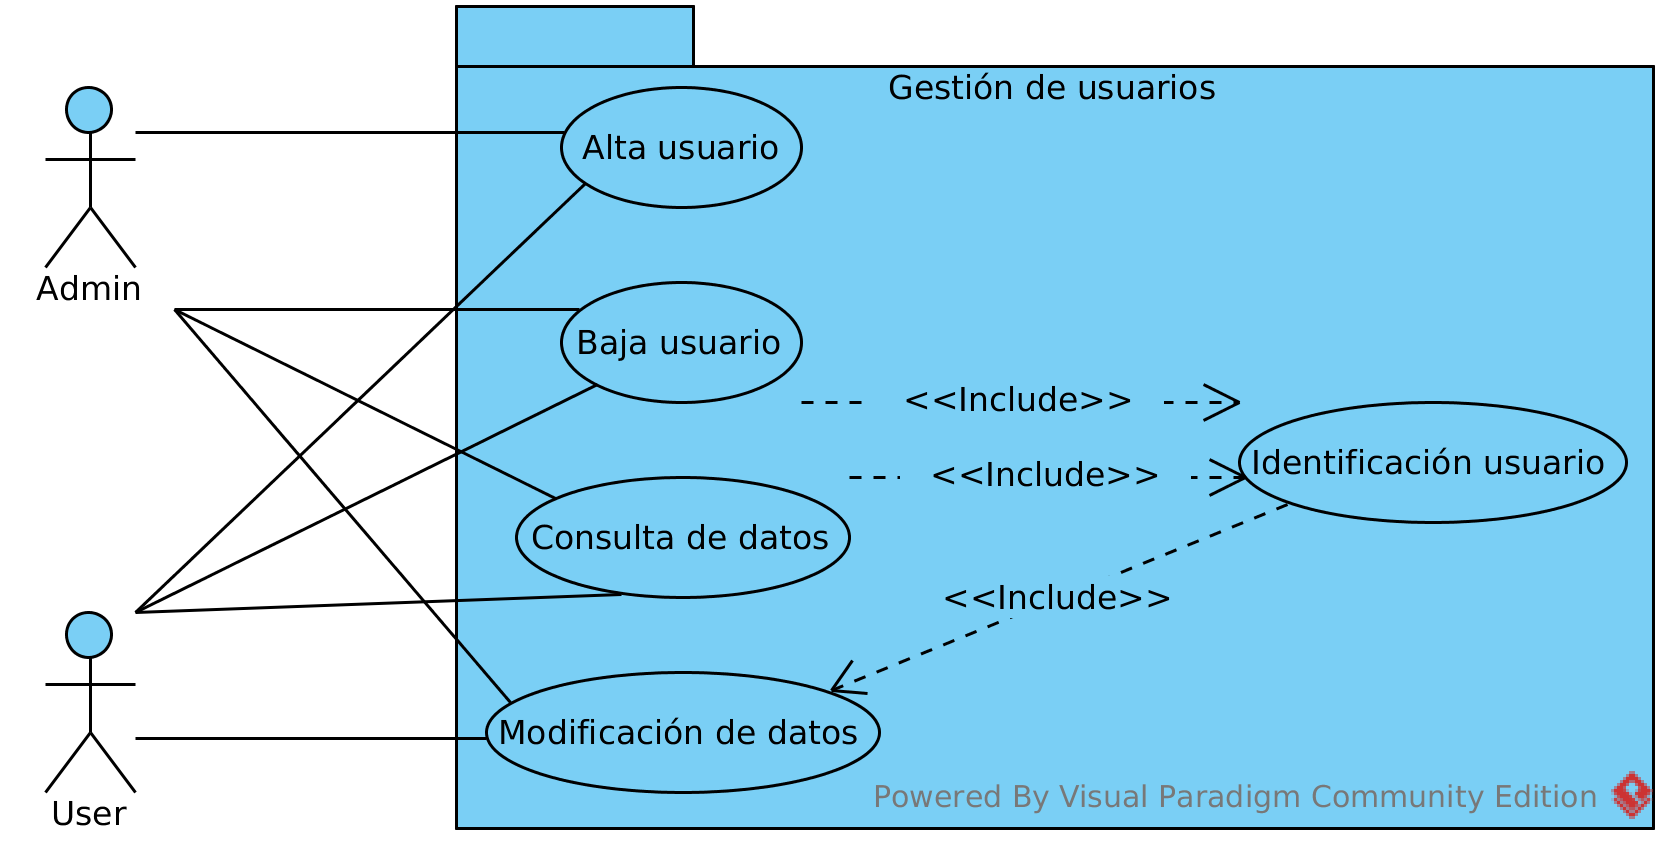
\includegraphics[width=0.65\textwidth]{../visual_paradigm_uml/CU-1_Gestion_de_usuarios.png}
  \caption{Diagrama de casos de uso. Gestión de usuarios}
  \label{fig:diag_cu_gu}
  \end{center}
\end{figure}

\begin{figure}[H]
  \begin{center}
  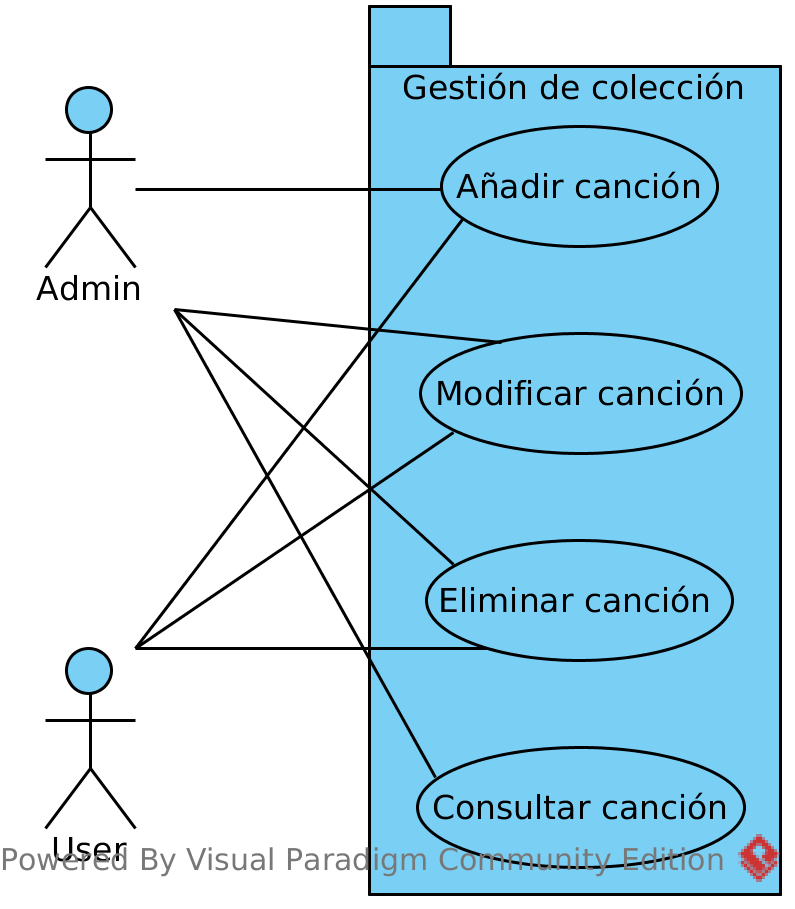
\includegraphics[width=0.4\textwidth]{../visual_paradigm_uml/CU-2_Gestion_de_canciones.png}
  \caption{Diagrama de casos de uso. Gestión de canciones}
  \label{fig:diag_cu_gc}
  \end{center}
\end{figure}

\begin{figure}[H]
  \begin{center}
  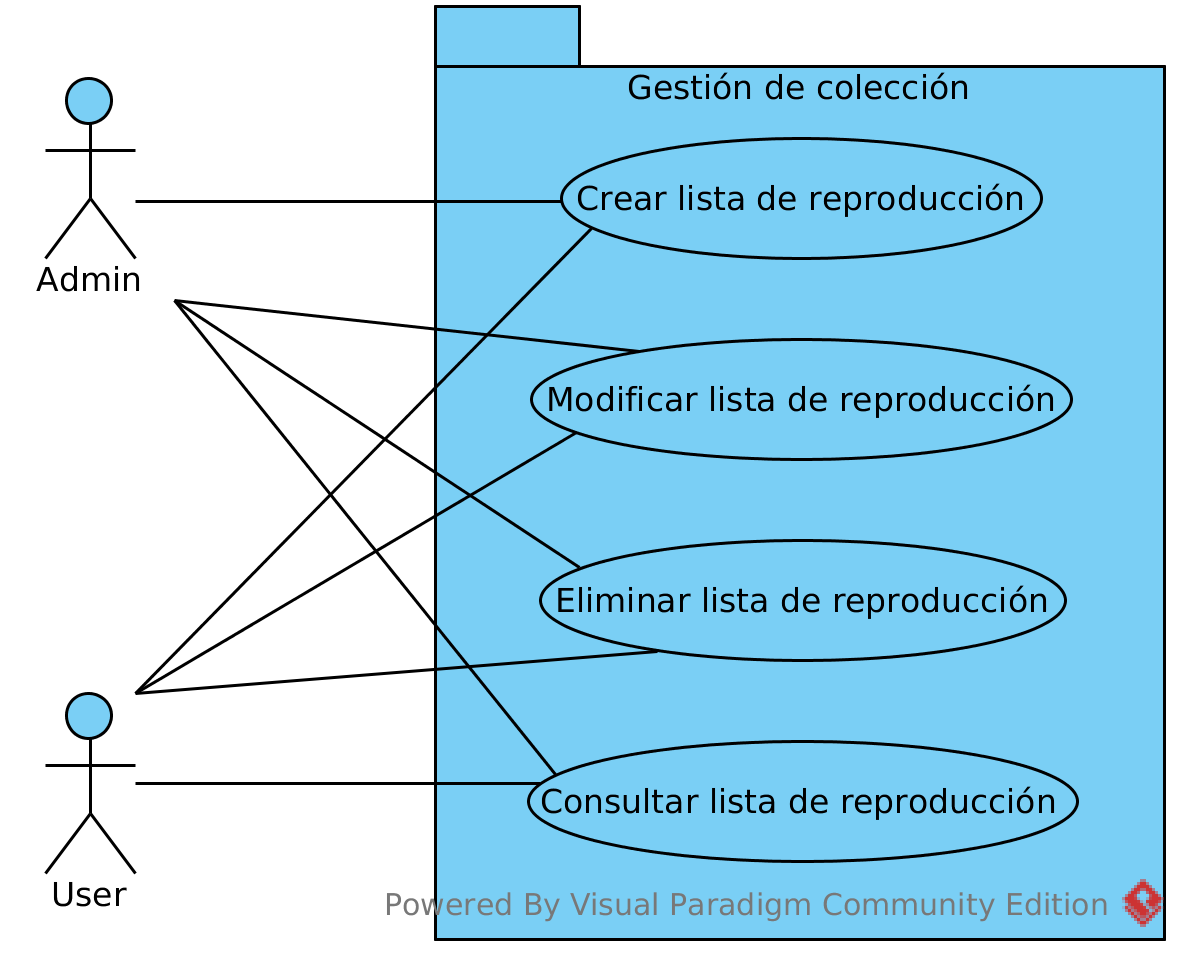
\includegraphics[width=0.65\textwidth]{../visual_paradigm_uml/CU-3_Gestion_de_listas_de_reproduccion.png}
  \caption{Diagrama de casos de uso. Gestión de listas de reproducción}
  \label{fig:diag_cu_glr}
  \end{center}
\end{figure}

\paragraph{Descripción de los casos de uso} \mbox{}

A continuación se exponen los casos de uso principales del sistema, correspondientes a las
acciones básicas del usuario con la plataforma, definiendo el comportamiento normal y
alternativo de cada acción.

% CASO DE USO 1
\textbf{CU-1.} Registro de usuarios (\textit{Sign Up}).
  
\begin{itemize}
    \item Descripción: el usuario se registrará con sus datos en el sistema.
    \item Precondición: el usuario no se encuentra registrado en el sistema.
    \item Postcondición: el usuario quedará registrado en el sistema con los datos proporcionados y se le asignará un identificador único.
\end{itemize}
    
\begin{table}[H]
  \begin{center}
    \begin{tabular}{|l|l|l|l|}
      \hline
      \multicolumn{4}{|c|}{{\bf Curso normal}}
      \\ \hline
      \multicolumn{2}{|c|}{{\bf Actor}} & \multicolumn{2}{|c|}{{\bf Sistema}}
      \\ \hline
      {\it 1} & 
      \begin{tabular}[c]{@{}l@{}}
        Usuario: inicia la acción\\
        de registro en el sistema.
      \end{tabular} &
      &
      \\ \hline
      &
      &
      {\it 2a} &
      \begin{tabular}[c]{@{}l@{}}
        Dar de alta al usuario en\\
        el sistema.
      \end{tabular}
      \\ \hline
      &
      &
      {\it 3} &
      \begin{tabular}[c]{@{}l@{}}
        El usuario queda dado de\\
        alta en el sistema y ya\\
        puede acceder.
      \end{tabular}
      \\ \hline
    \end{tabular}
    \caption{Curso normal de CU-1. Registro de usuarios.}
    \label{table:cn_cu_1}
  \end{center}
\end{table}

\begin{table}[H]
  \begin{center}
    \begin{tabular}{|l|l|}
      \hline
      \multicolumn{2}{|c|}{{\bf Curso alterno}}
      \\ \hline
      {\it 2b} &
      \begin{tabular}[c]{@{}l@{}}
        Si alguno de los datos que identifican al usuario se encuentran\\
        ya registrados en el sistema o alguno de ellos es inválido, no\\
        se continúa y se notifica el error al usuario.
      \end{tabular}\\
      \hline
    \end{tabular}
    \caption{Curso alterno de CU-1. Registro de usuarios.}
    \label{table:ca_cu_1}
  \end{center}
\end{table}

% CASO DE USO 2
\textbf{CU-2.} Identificación de usuarios (\textit{Log In}).

\begin{itemize}
    \item Descripción: el usuario iniciará con sus datos de acceso una sesión en el sistema.
    \item Precondición: el usuario se encuentra registrado en el sistema
    \item Postcondición: el usuario obtiene acceso al sistema y queda identificado en él, iniciándose su sesión.
\end{itemize}

\begin{table}[H]
  \begin{center}
    \begin{tabular}{|l|l|l|l|}
      \hline
      \multicolumn{4}{|c|}{{\bf Curso normal}}
      \\ \hline
      \multicolumn{2}{|c|}{{\bf Actor}} & \multicolumn{2}{|c|}{{\bf Sistema}}
      \\ \hline
      {\it 1} & 
      \begin{tabular}[c]{@{}l@{}}
        Usuario: inicia sesión.
      \end{tabular} &
      &
      \\ \hline
      &
      &
      {\it 2a} &
      \begin{tabular}[c]{@{}l@{}}
        Inicia la sesión del usuario\\
        en el sistema y genera un hash\\
        con el id de sesión que se enviará\\
        al usuario.
      \end{tabular}
      \\ \hline
      &
      &
      {\it 3} &
      \begin{tabular}[c]{@{}l@{}}
        El usuario queda logeado\\
        en el sistema y ya\\
        puede acceder.
      \end{tabular}
      \\ \hline
    \end{tabular}
    \caption{Curso normal de CU-2. Identificación de usuarios.}
    \label{table:cn_cu_2}
  \end{center}
\end{table}

\begin{table}[H]
  \begin{center}
    \begin{tabular}{|l|l|}
      \hline
      \multicolumn{2}{|c|}{{\bf Curso alterno}}
      \\ \hline
      {\it 2b} &
      \begin{tabular}[c]{@{}l@{}}
        Si alguno de los datos que identifican al usuario no coinciden\\
        con los almacenados en el sistema o alguno de ellos es inválido,\\
        no se continúa y se notifica el error al usuario.
      \end{tabular}\\
      \hline
    \end{tabular}
    \caption{Curso alterno de CU-2. Identificación de usuarios.}
    \label{table:ca_cu_2}
  \end{center}
\end{table}

% CASO DE USO 3
\textbf{CU-3.} Añadir canción.
  
\begin{itemize}
    \item Descripción: se añade una canción a la colección del usuario.
    \item Precondición: el usuario se encuentra con una sesión iniciada en el sistema
    \item Postcondición: se vincula la canción subida al usuario cuya sesión se encontraba iniciada en el momento de subirse a la plataforma.
\end{itemize}

\begin{table}[H]

  \begin{center}
    \begin{tabular}{|l|l|l|l|}
      \hline
      \multicolumn{4}{|c|}{{\bf Curso normal}}
      \\ \hline
      \multicolumn{2}{|c|}{{\bf Actor}} & \multicolumn{2}{|c|}{{\bf Sistema}}
      \\ \hline
      {\it 1} & 
      \begin{tabular}[c]{@{}l@{}}
        Usuario: selecciona un fichero\\
        de audio para subirlo a la\\
        plataforma.
      \end{tabular} &
      &
      \\ \hline
      &
      &
      {\it 2a} &
      \begin{tabular}[c]{@{}l@{}}
        El fichero se sube al sistema\\ 
        y se procesa.
      \end{tabular}
      \\ \hline
      &
      &
      {\it 3} &
      \begin{tabular}[c]{@{}l@{}}
        La canción queda vinculada\\
        con el usuario y se añade\\
        como parte de su colección.
      \end{tabular}
      \\ \hline
    \end{tabular}
    \caption{Curso normal de CU-3. Añadir canción.}
    \label{table:cn_cu_3}
  \end{center}
\end{table}

\begin{table}[H]
  \begin{center}
    \begin{tabular}{|l|l|}
      \hline
      \multicolumn{2}{|c|}{{\bf Curso alterno}}
      \\ \hline
      {\it 2b} &
      \begin{tabular}[c]{@{}l@{}}
        Si el formato del fichero no es válido o se cancela la subida por\\
        cualquier motivo, la canción no se añade al sistema y se notifica\\
        al usuario el error.
      \end{tabular}\\
      \hline
    \end{tabular}
    \caption{Curso alterno de CU-3. Añadir canción.}
    \label{table:ca_cu_3}
  \end{center}
\end{table}

% CASO DE USO 4
\textbf{CU-4.} Consultar canción.
  
\begin{itemize}
    \item Descripción: se muestran los datos solicitados de una canción.
    \item Precondición: el usuario se encuentra con una sesión iniciada en el sistema.
    \item Postcondición: el sistema devuelve los datos.
\end{itemize}

\begin{table}[H]

  \begin{center}
    \begin{tabular}{|l|l|l|l|}
      \hline
      \multicolumn{4}{|c|}{{\bf Curso normal}}
      \\ \hline
      \multicolumn{2}{|c|}{{\bf Actor}} & \multicolumn{2}{|c|}{{\bf Sistema}}
      \\ \hline
      {\it 1} & 
      \begin{tabular}[c]{@{}l@{}}
        Usuario: selecciona una canción para\\
        consultar sus datos.
      \end{tabular} &
      &
      \\ \hline
      &
      &
      {\it 2a} &
      \begin{tabular}[c]{@{}l@{}}
        Busca la canción en el\\
        sistema y devuelve sus\\
        datos al usuario.
      \end{tabular}
      \\ \hline
    \end{tabular}
    \caption{Curso normal de CU-4. Consultar canción.}
    \label{table:cn_cu_4}
  \end{center}
\end{table}

\begin{table}[H]
  \begin{center}
    \begin{tabular}{|l|l|}
      \hline
      \multicolumn{2}{|c|}{{\bf Curso alterno}}
      \\ \hline
      {\it 2b} &
      \begin{tabular}[c]{@{}l@{}}
        Si la canción que intenta pedir el usuario no existe en la base\\
        de datos o no pertene al usuario, no se devuelven sus datos y se\\
        informa del error.
      \end{tabular}\\
      \hline
    \end{tabular}
    \caption{Curso alterno de CU-4. Consultar canción.}
    \label{table:ca_cu_4}
  \end{center}
\end{table}

% CASO DE USO 5
\textbf{CU-5.} Modificar canción.
  
\begin{itemize}
    \item Descripción: se actualizan los atributos que se han modificado en la canción.
    \item Precondición: el usuario se encuentra con una sesión iniciada en el sistema.
    \item Postcondición: el sistema actualiza los datos de la canción.
\end{itemize}

\begin{table}[H]

  \begin{center}
    \begin{tabular}{|l|l|l|l|}
      \hline
      \multicolumn{4}{|c|}{{\bf Curso normal}}
      \\ \hline
      \multicolumn{2}{|c|}{{\bf Actor}} & \multicolumn{2}{|c|}{{\bf Sistema}}
      \\ \hline
      {\it 1} & 
      \begin{tabular}[c]{@{}l@{}}
        Usuario: selecciona una canción\\
        para modificar sus datos.
      \end{tabular} &
      &
      \\ \hline
      &
      &
      {\it 2a} &
      \begin{tabular}[c]{@{}l@{}}
        Busca la canción en el sistema\\
        y devuelve un formulario con\\
        los datos actuales para que\\
        el usuario modifique los que\\
        considere oportunos.
      \end{tabular}
      \\ \hline
      {\it 3a} & 
      \begin{tabular}[c]{@{}l@{}}
        Usuario: modifica algún dato\\
        del formulario y lo envía.
      \end{tabular} &
      &
      \\ \hline
      &
      &
      {\it 4a} &
      \begin{tabular}[c]{@{}l@{}}
        Actualiza la canción con los\\
        nuevos datos y lo envía al\\
        usuario de vuelta para que\\
        los visualice.
      \end{tabular}
      \\ \hline
    \end{tabular}
    \caption{Curso normal de CU-5. Modificar canción.}
    \label{table:cn_cu_5}
  \end{center}
\end{table}

\begin{table}[H]
  \begin{center}
    \begin{tabular}{|l|l|}
      \hline
      \multicolumn{2}{|c|}{{\bf Curso alterno}}
      \\ \hline
      {\it 2b} &
      \begin{tabular}[c]{@{}l@{}}
        Si la canción que intenta pedir el usuario no existe en la base\\
        de datos o no pertene al usuario, no se devuelven sus datos y se\\
        informa del error.
      \end{tabular}\\
      \hline
      {\it 3b} &
      \begin{tabular}[c]{@{}l@{}}
        Si el usuario cancela la edición de los datos, se termina el proceso\\
        y no se continúa.
      \end{tabular}\\
      \hline
      {\it 4b} &
      \begin{tabular}[c]{@{}l@{}}
        Si alguno de los datos introducidos no es válido, se le notifica al\\
        usuario y se vuelve al punto 3a.
      \end{tabular}\\
      \hline
    \end{tabular}
    \caption{Curso alterno de CU-5. Modificar canción.}
    \label{table:ca_cu_5}
  \end{center}
\end{table}

% CASO DE USO 6
\textbf{CU-6.} Eliminar canción.
  
\begin{itemize}
    \item Descripción: se elimina del sistema la canción seleccionada.
    \item Precondición: el usuario se encuentra con una sesión iniciada en el sistema.
    \item Postcondición: el sistema elimina los datos de la canción, el fichero asociado y su imagen (en caso de que tenga).
\end{itemize}

\begin{table}[H]

  \begin{center}
    \begin{tabular}{|l|l|l|l|}
      \hline
      \multicolumn{4}{|c|}{{\bf Curso normal}}
      \\ \hline
      \multicolumn{2}{|c|}{{\bf Actor}} & \multicolumn{2}{|c|}{{\bf Sistema}}
      \\ \hline
      {\it 1} & 
      \begin{tabular}[c]{@{}l@{}}
        Usuario: selecciona una canción para\\
        eliminar de su colección.
      \end{tabular} &
      &
      \\ \hline
      &
      &
      {\it 2a} &
      \begin{tabular}[c]{@{}l@{}}
        Busca la canción en el \\
        sistema y elimina todos\\
        sus datos, desvinculándose\\
        de la colección del usuario.
      \end{tabular}
      \\ \hline
    \end{tabular}
    \caption{Curso normal de CU-6. Eliminar canción.}
    \label{table:cn_cu_6}
  \end{center}
\end{table}

\begin{table}[H]
  \begin{center}
    \begin{tabular}{|l|l|}
      \hline
      \multicolumn{2}{|c|}{{\bf Curso alterno}}
      \\ \hline
      {\it 2b} &
      \begin{tabular}[c]{@{}l@{}}
        Si la canción que intenta pedir el usuario no existe en la base\\
        de datos o no pertene al usuario, no se eliminan sus datos y se\\
        informa del error.
      \end{tabular}\\
      \hline
    \end{tabular}
    \caption{Curso alterno de CU-6. Eliminar canción.}
    \label{table:ca_cu_6}
  \end{center}
\end{table}

% CASO DE USO 7,8,9,10

\textbf{CU-7, CU-8, CU-9, CU-10} CRUD listas de reproducción.\\

Los casos de uso correspondientes a la creación, consulta, actualización y borrado de listas de reproducción son análogos a los descritos para el caso de las canciones.

\subsubsection{Diagramas de actividad}

Los diagramas de actividad representan la descomposición de un proceso en las diferentes subacciones y estados en los que se apoya. A continuación se muestra un diagrama de actividad que representa el flujo que pueden seguir las acciones del usuario en el sistema.

\begin{figure}[H]
  \begin{center}
  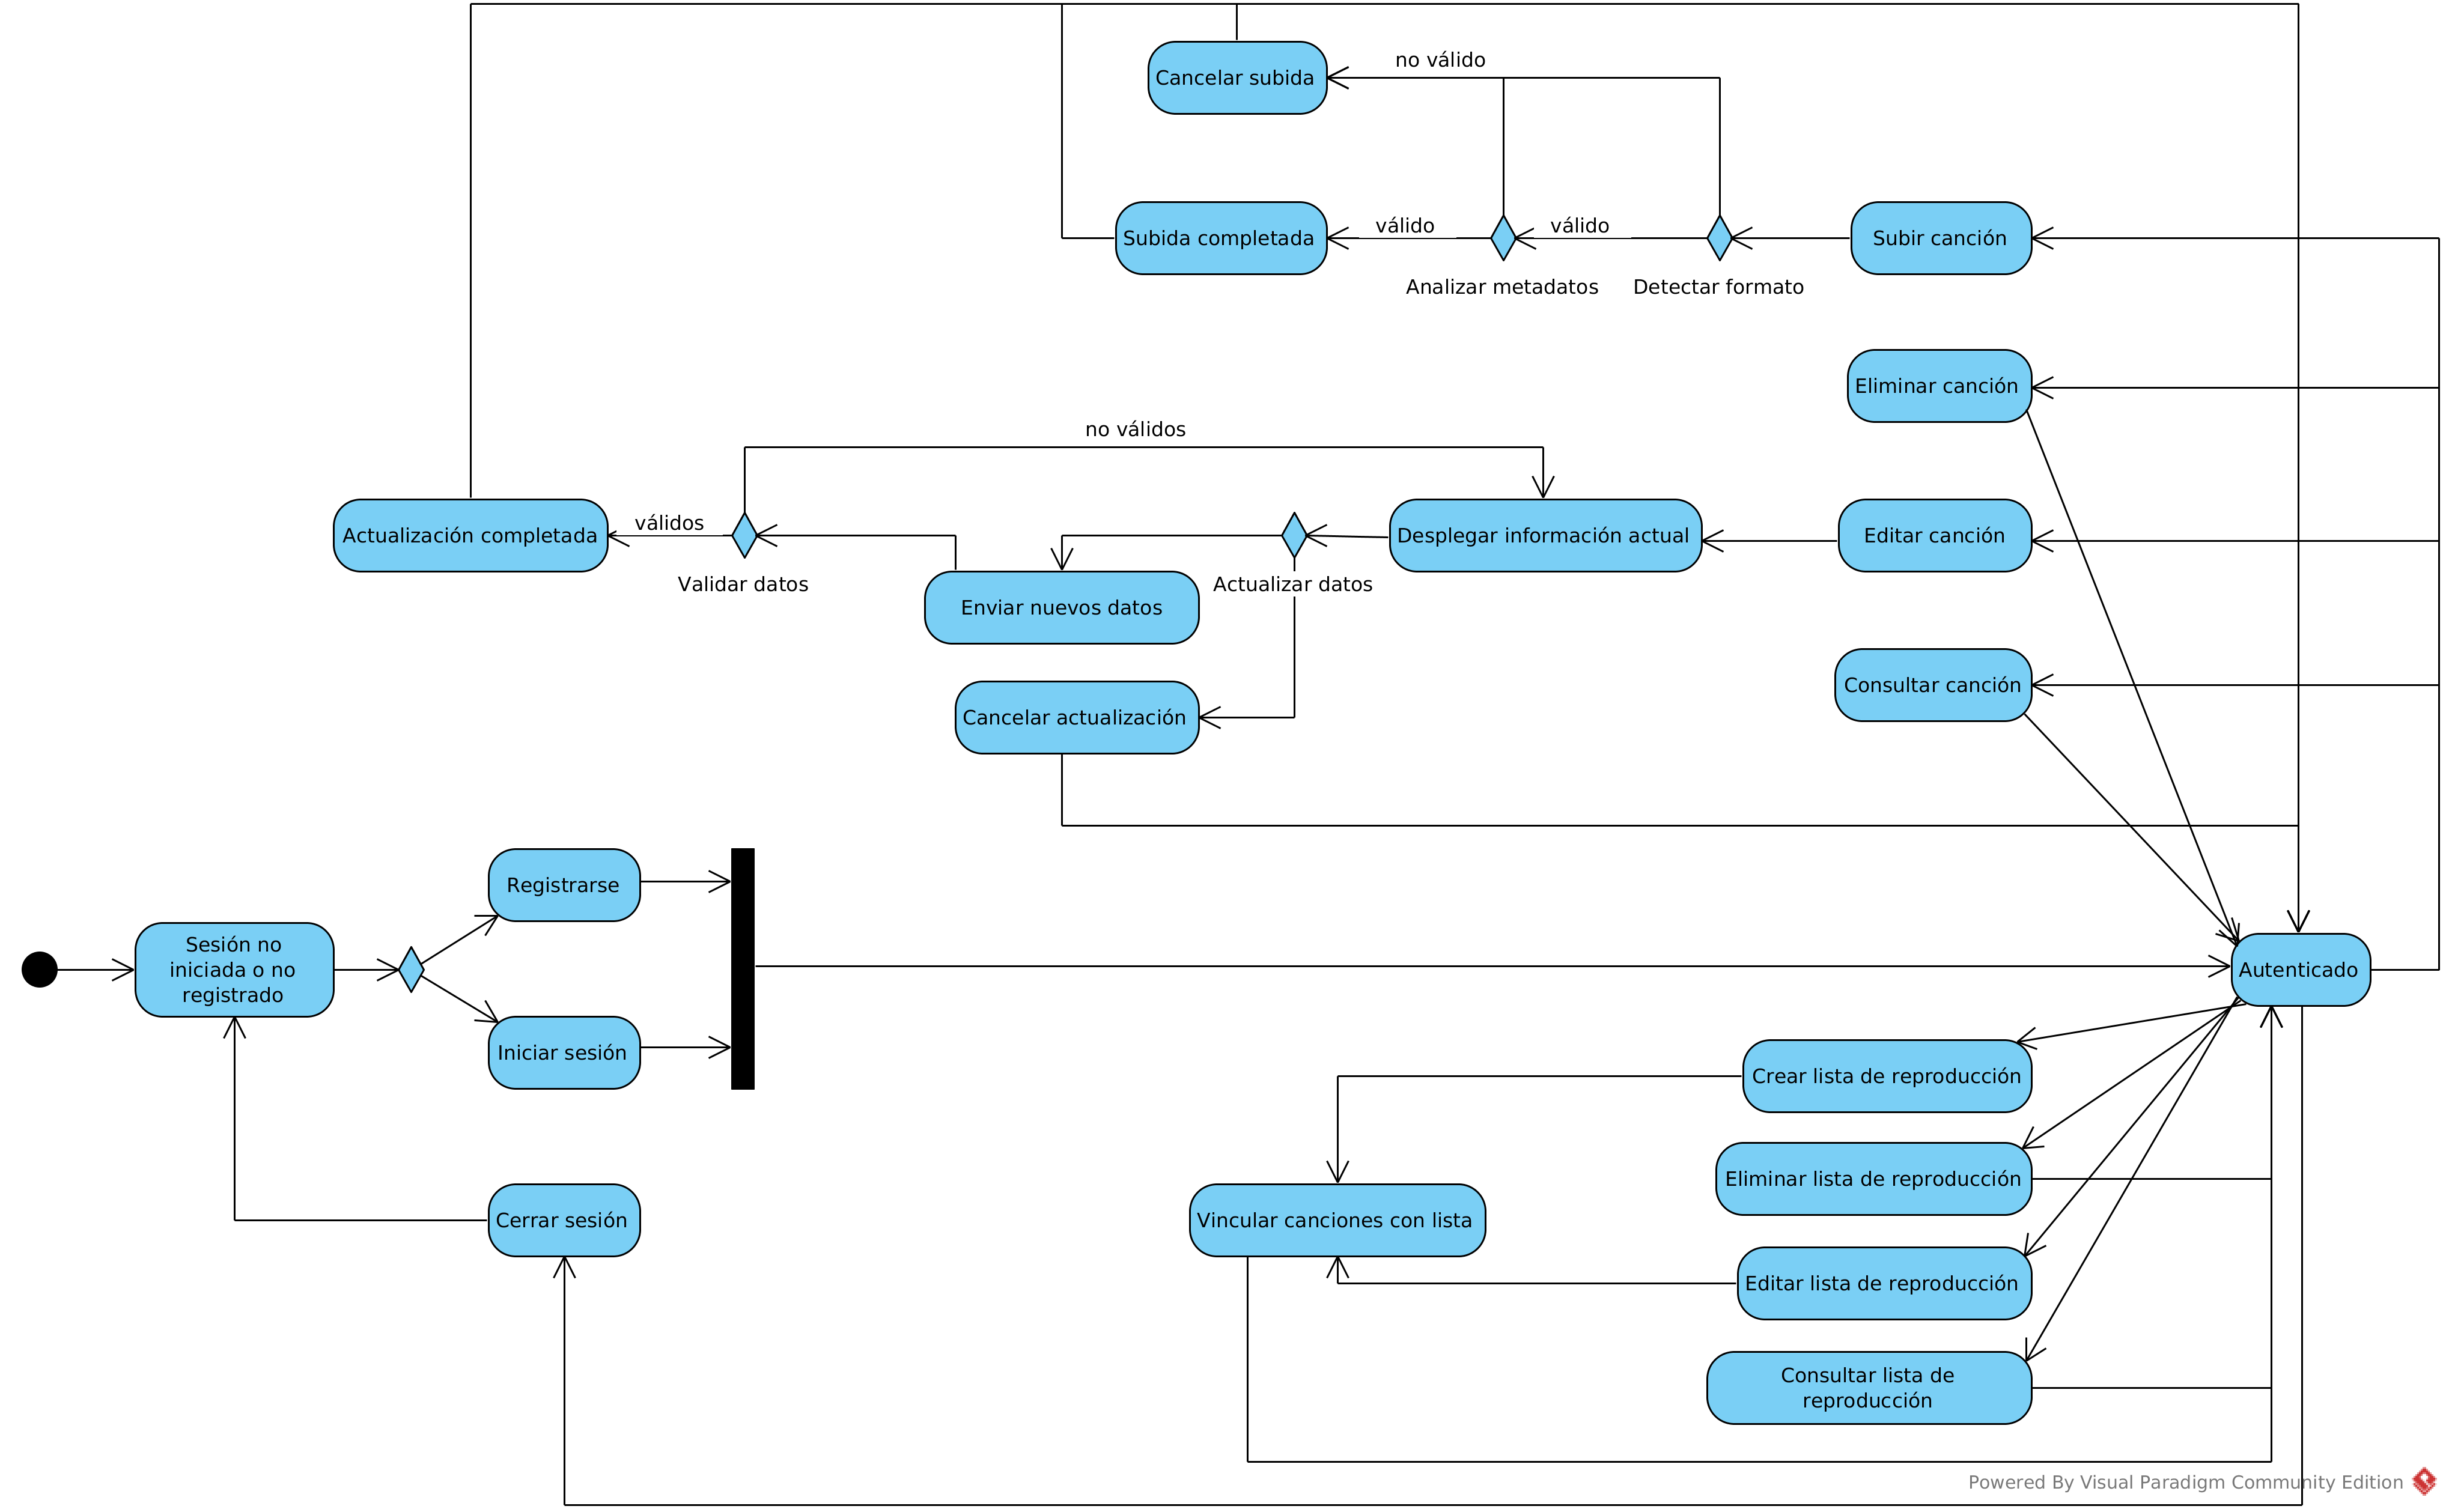
\includegraphics[width=1\textwidth]{../visual_paradigm_uml/Diagrama_actividad_sistema.png}
  \caption{Diagrama de actividad del sistema}
  \label{fig:diag_ac_sis}
  \end{center}
\end{figure}

\subsubsection{Diagrama de clases del diseño}

En el diagrama de clases del diseño se muestra la especificación para las clases software de la aplicación e incluye:

\begin{itemize}
    \item Clases, asociaciones y atributos
    \item Métodos
    \item Navegabilidad
    \item Dependencias
\end{itemize}

A continuación se muestra el diagrama de clases del diseño propuesto:

\begin{figure}[H]
  \begin{center}
  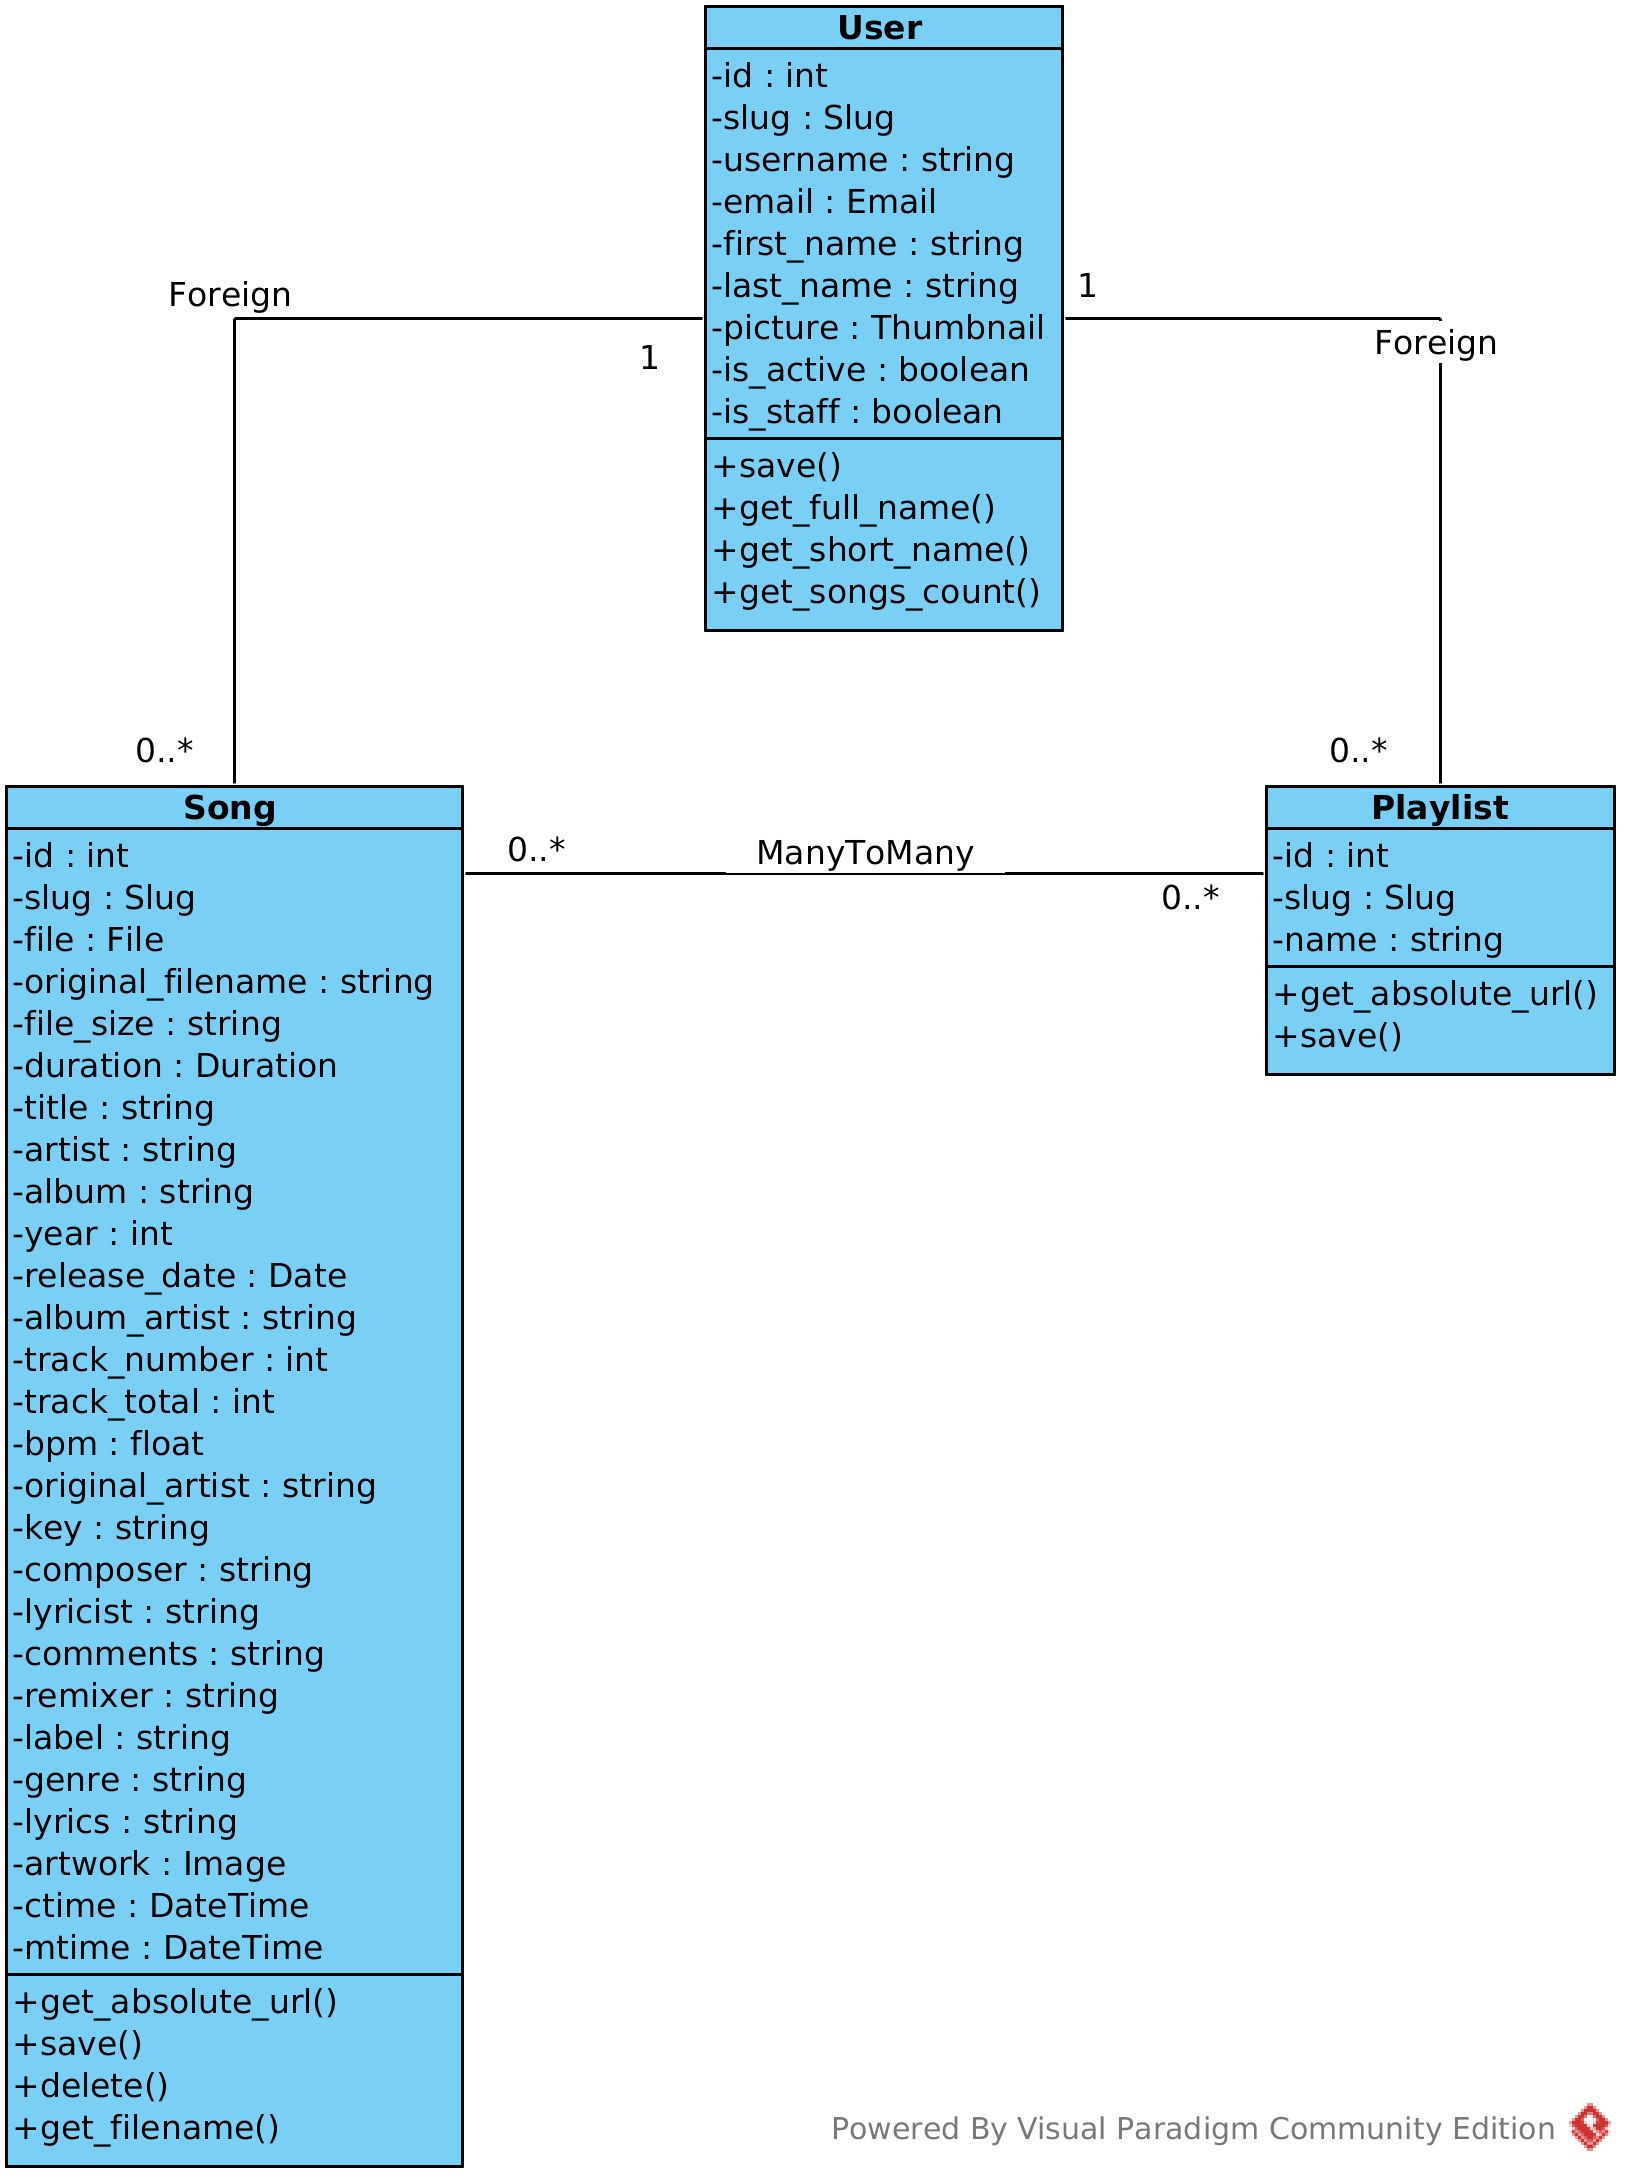
\includegraphics[width=0.8\textwidth]{../visual_paradigm_uml/Diagrama_clases.png}
  \caption{Diagrama de clases del diseño}
  \label{fig:diag_class}
  \end{center}
\end{figure}


\chapter{Diseño}
\label{cap:disenio}

En esta sección se especificarán los aspectos más relevantes para el desarrollo del sistema: tecnologías a utilizar, cómo y por qué utilizarlas, etc. A continuación se profundizará en las herramientas a utilizar en cada una de las partes de la plataforma web y, para una mejor comprensión, dividiremos este apartado en tres: servidor (\textit{backend}), cliente (\textit{frontend}) e infraestructura.

\section{Backend}

\subsection{Patrón Modelo-Vista-Controlador}

Para el desarrollo se plantea basarse en el patrón de arquitectura software Modelo-Vista-Controlador (MVC), cuyos principios se basan en separar los datos y la lógica de la aplicación de su interfaz, con el objetivo de facilitar el desarrollo y mantenimiento de la aplicación. De este modo, distinguimos los siguientes componentes:

\begin{itemize}
    \item \textbf{Modelo}: representa la información con la que opera el sistema. Gestiona los accesos a dicha información, como consultas y actualizaciones. Se encarga de enviar a la vista la información que solicite para su visualización. Las peticiones de acceso a dicha información llegan a éste a través del controlador.
    \item \textbf{Vista}: presenta el modelo en el formato adecuado. En este caso, la vista es el \textit{frontend} de nuestra aplicación.
    \item \textbf{Controlador}: responde a los eventos, invoca peticiones al modelo para solicitar información y puede enviar comandos a su vista asociada.
\end{itemize}

Una vez presentado el patrón, debemos buscar una tecnología que se adapte a este. Finalmente, nos decantaremos por Django, un framework de alto nivel para trabajar con python en el servidor.

\subsection{Django} \cite{Dj}
Como decíamos, Django se trata de un framework de desarrollo web a alto nivel y de código abierto (licencia BSD), escrito en Python y que representa el patrón de diseño Modelo-vista-controlador. Su meta fundamental es facilitar la creación de sitios web complejos, haciéndo énfasis en la reutilización, conectividad y extensibilidad de componentes, el desarrollo ágil y el principio No te repitas (DRY, del inglés \textit{Don't Repeat Yourself}). A continuación se exponen algunas de las razones por las que elegir a Django frente a otros frameworks de desarrollo web.

\begin{itemize}
    \item ORM: se trata de una potente herramienta de base de datos. Basándose en los modelos que el usuario codifique, Django es capaz de convertirlos a una base de datos orientada a objetos. Además, se ofrece soporte a diversos Sistemas Gestores de Base de Datos (MySQL, MariaDB, PostgreSQL, Oracle y SQLite), unificados bajo una misma sintaxis y dejando de lado a SQL como lenguaje de consultas.
    \item Formularios: Gracias a Django la validación de formularios es mucho más sencilla. Solamente tienes que definir los atributos de tus modelos y como quieres que funcione la validación básica.
    \item Panel de administración: Django ofrece un panel de administración altamente personalizable que puede incluso utilizarse como area de administración final en tu aplicación web.
    \item Django no es PHP: para aquellos que busquen un cambio, Django es una gran alternativa a PHP, además de tener una gran comunidad de usuarios detrás.
    \item Django es Python, un lenguaje de scripting elegante y potente con una gran comunidad de usuarios detrás.
    \item Proyectos existosos construidos en Django \cite{SUDj}: 
    \begin{itemize}
        \item Disqus \cite{Disqus}: plataforma que ofrece un sistema de discusiones para tu blog o sitio web.
        \item Instagram \cite{Instagram}: la aplicación más famosa para subir imágenes y aplicar efectos en ellas.
        \item Open Stack \cite{Open Stack}: proyecto de computación en la nube que proporciona una Infraestructura Como Servicio (IaaS).
        \item Pinterest \cite{Pinterest}: red social para compartir imágenes que permite a los usuarios crear y administrar en tableros personales temáticos colecciones de imágenes, como eventos, intereses o aficiones entre otros.
    \end{itemize}
\end{itemize}

\subsubsection{Modelo-Template-Vista}
Un aspecto a tener en cuenta en Django, es que no representa el patrón Modelo-vista-controlador como tal, si no que se basa en lo que podríamos denominar ``Modelo-template-vista''. Si bien es cierto que se asemeja mucho a la implementación del patrón MVC, para Django la Vista describe ``qué'' datos serán presentados y no ``cómo'' se verán los mismos, siéndo los \textit{templates} los encargados de esta última tarea.

Esto se debió a que los desarrolladores del framework no buscaron apegarse a nada en particular, sino desarrollar una herramienta que funcionara lo mejor posible.

\begin{figure}[H]
  \begin{center}
  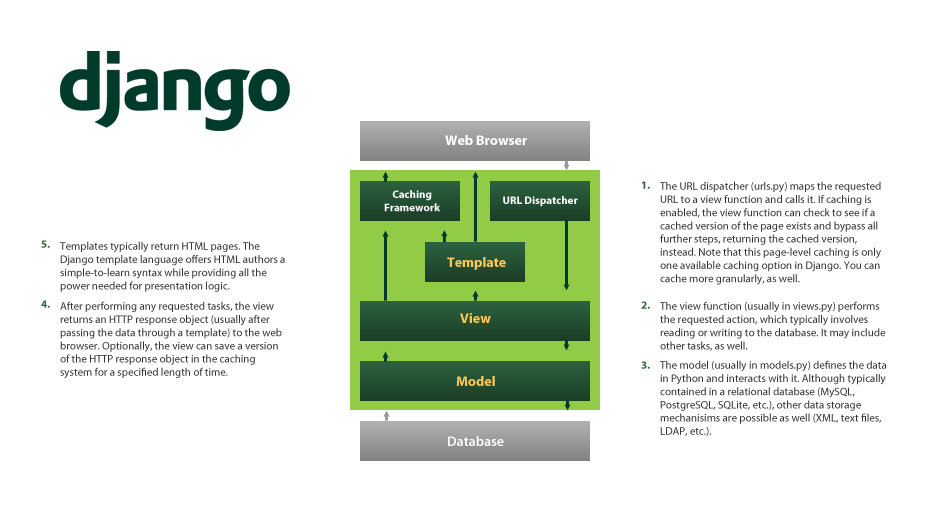
\includegraphics[width=0.8\textwidth]{../images/django_arch.png}
  \caption{Arquitectura de Django}
  \label{fig:django_arch}
  \end{center}
\end{figure}

\subsubsection{Sistema Gestor de Base de Datos}
El Sistema Gestor de Base de Datos es el encargado de proporcionar la capa de acceso a la información de la base de datos. Como hemos comentado, haciendo uso del ORM de Django, utilizaremos un conector para base de datos SQLite durante el desarrollo, que se modificará por un MySQL o postgreSQL para las fases de ``puesta en marcha'' (\textit{staging}) y producción.

\section{Frontend}
El \textit{frontend} es la capa de presentación de la aplicación, encargada de maquetar la estructura semántica del contenido (HTML), codificar el diseño en hojas de estilo (CSS) y agregar la interacción con el usuario (Javascript). En este proyecto, el cliente representará un papel bastante importante con respecto a la experiencia del usuario en la plataforma. Por ello, se trabajará además con una librería de Javascript, jQuery, que nos ayudará a dicho propósito, facilitando algunas tareas. 

\subsection{jQuery y AJAX}
Como comentábamos, jQuery \cite{jQuery} es una librería de Javascript, que facilita la interacción con los documentos HTML mediante la manipulación del árbol DOM y cuyo principal objetivo es dotar a la web de un comportamiento dinámico. Además, destacar que es compatible con la mayoría de navegadores actuales y la última versión de CSS (CSS3).

La principal ventaja de jQuery frente a otros competidores como Flash es su excelente integración con AJAX.

AJAX (\textit{Asynchronous Javascript and XML}) \cite{AJAX} consiste en una técnica de desarrollo web para generar aplicaciones interactivas que se ejecutan del lado cliente de manera que es posible realizar cambios en las páginas sin necesidad de recargarlas, mejorando consecuentemente la interactividad, velocidad y usabilidad de las aplicaciones.

En definitiva, el uso de estas tecnologías permitirán mejorar la experiencia de usuario mientras este navegue por el sistema.

\subsection{Twitter Bootstrap}
Otro aspecto a tener en cuenta de cara al lado del cliente de nuestra aplicación, es su diseño. Para ello, nos apoyaremos en Twitter Bootstrap \cite{Bootstrap}, un framework CSS que facilita la tarea de dar forma al sitio web. De esta forma, podremos crear interfaces de usuario elegantes y limpias además de responder a un diseño adaptativo según dispositivos y pantallas de forma muy sencilla.

\section{Infraestructura}

Por último, para alojar el código de nuestra aplicación y dotar al sistema de las diferentes funcionalidades, haremos uso de Github.

\subsection{Github}

Github \cite{Github} es una plataforma de desarrollo colaborativo que permite alojar proyectos mediante el sistema de control de versiones Git \cite{Git}. El código puede almacenarse tanto de forma pública como privada (opción de pago), y es alojado en repositorios que brindan las siguientes características:

\begin{itemize}
	\item Una wiki para cada proyecto.
	\item Una página web para cada proyecto (\textit{Github Pages}).
	\item Sistema de seguimiento de errores (\textit{issues}).
	\item Gráfico que muestra cómo trabajan los desarrolladores en el repositorio y bifurcaciones del proyecto.
	\item Funcionalidades de red social
\end{itemize}

De esta forma, se ha creado una organización dentro de la plataforma en \url{https://github.com/hearcloud} que alojará los repositorios asociados al proyecto, en este caso:

\begin{itemize}
	\item Repositorio para el código del proyecto: \url{https://github.com/hearcloud/hearcloud}.
	\item Repositorio para la documentación en {\LaTeX\xspace}: \url{https://github.com/hearcloud/hearcloud-doc}
\end{itemize}

\subsection{Travis-CI}

\subsection{Plataforma Como Servicio}

\subsubsection{Openshift}

\subsection{Provisionamiento: Ansible}

\subsection{Ejecución automática de comandos en remoto. Fabric}



\chapter{Implementación}
\label{cap:implementacion}

Tras el estudio en el capítulo anterior de las herramientas apropiadas para el desarrollo del prototipo de nuestra aplicación, pasamos a describir en éste los aspectos propios, ya si, de su implementación. Lo primero a analizar será la estructura de nuestro proyecto en Django.

\section{Estructura del proyecto}

\subsection{Aplicaciones}

\subsubsection{Home}

\subsubsection{Users}

\subsubsection{Box}

\subsection{URLs}

\subsection{Archivos estáticos}

\section{Dependencias}

\subsection{Pillow}

\subsection{Django Cors Headers}

\subsection{Django FM}

\subsection{Django Rest Framework}

\subsubsection{Django Rest Auth}

\subsubsection{Django Allauth}

\subsection{Mutagen}

\subsection{pyDub}

\subsubsection{ffmpeg}

\subsection{Humanize}

\chapter{Pruebas}
\label{cap:pruebas}


\chapter{Conclusiones y trabajos futuros}
\label{cap:conclusiones}

\section{Conclusiones}

Tras finalizar el proyecto, hemos obtenido un \textit{prototipo funcional} de la aplicación que habíamos especificado en un principio, así como una memoria correctamente documentada sobre el desarrollo del mismo.

En base a las primeras pruebas de despliegue, el prototipo desarrollado presenta un conjunto de tecnologías e infraestructura viables para resolver el problema planteado, permitiendo así un desarrollo posterior.

Hearcloud concluye como un sistema \textit{open source} para la gestión de la bilbioteca musical de sus usuarios, resultado de 7 meses de desarrollo listo para su implantación en cualquier arquitectura.

\subsection{Conocimientos adquiridos}
Gracias al análisis y desarrollo de este proyecto, se han ido adquiriendo conocimientos en diversos ámbitos del desarrollo de software, sobre todo, en el ámbito de las tecnologías web, entre las que destacamos:

\begin{itemize}
	\item Profundización en el conocimiento del lenguaje de programación Python y librerías asociadas al tratamiento de audio, así como del framework para desarrollo web Django.
	\item Técnicas para el desarrollo de interfaces de aplicaciones \textit{frontend} mediante tecnologías web modernas como \textit{Bootstrap}, \textit{jQuery} y \textit{AJAX}.
	\item Habilidades para la gestión de proyectos software de tamaño medio aplicando técnicas de desarrollo viables.
	\item Desarrollo de pruebas automatizadas que comprueben la calidad del software generado
	\item Técnicas \textit{DevOps} para la aplicación de un flujo de desarrollo con testeo y despligue automáticos mediante integración continua.
\end{itemize} 

\subsection{Materias cursadas relacionadas con el proyecto}

El proyecto aplica conocimientos adquiridos en diversas asignaturas relacionadas con la titulación, tanto generales como de la especialidad en Tecnologías de la Información.

\begin{itemize}
	\item Materias relacionadas con los fundamentos de programación \cite{FP} \cite{MP} y Programación y Diseño Orientado a Objetos \cite{PDOO}.
	\item Fundamentos de Bases de Datos \cite{FBD}, Estructura de Datos \cite{ED}, Diseño y Desarrollo de Sistemas de Información \cite{DDSI} y Fundamentos de Ingeniería del Software \cite{FIS}.
	\item Tecnologías de la Información: Desarrollo de Aplicaciones para Internet \cite{DAI} e Infraestructura Virtual \cite{IV}.
\end{itemize}

\section{Trabajos futuros}
Si bien el prototipo resuelve los problemas iniciales planteados, aún dista de ser un software listo para producción competente de acuerdo a las exigencias del mercado actuales, por lo que se abren diferentes líneas de trabajo orientadas al desarrollo de un producto completo.

\begin{itemize}
	\item Mejoras en cuanto a la eficiencia de la interfaz de usuario en el lado del cliente.
	\item Mejoras en las funcionalidades existentes e inclusión de otras nuevas (envío de emails, soporte para nuevos formatos de audio, etc).
	\item Creación de clientes móviles y de escritorio en las diferentes plataformas.
\end{itemize}

Teniendo en cuenta todo esto, se realiza una estimación preliminar para un tiempo de desarrollo adicional de seis meses con un equipo de desarrollo de entre cuatro a seis desarrolladores para obtener dicha versión completa del producto.

\subsection{Angular}
Angular \cite{Angular} es un framework Javascript de código abierto, mantenido por Google, que se utiliza para crear lo que se denomina páginas web de una sola página \cite{SPA}. Aunque su versión 2.0 se encuentra aún en fase de pruebas frente a la actual 1.5.8, está encaminada a convertirse en todo un estándar y una tecnología muy a tener en cuenta para abordar desarrollos del lado del cliente.

Se plantea la posibilidad de portar el \textit{frontend} desarrollado durante el transcurso de este proyecto a una aplicación Angular, apostando por su versión 2 que incluye diversos cambios y mejoras, entre los que destacamos:

\begin{itemize}
	\item Enfocado a Web Components \cite{WC}. Se trata de un conjunto de especificaciones que indican cómo deben de desarrollarse webs a día de hoy.
	\item \textit{Mobile First Design}. Representa mejoras de rendimiento en terminales móviles.
	\item Detección de cambios en las vistas optimizada.
	\item Inyección de dependencias reescrita completamente para mejorar la gestión de memoria y la seguridad en el acceso a las distintas instancias que se solicitan
	\item Apuesta por TypeScript \cite{Typescript}, que es una extensión de Javascript que cuenta con interesantes características y mejoras:
	\begin{itemize}
		\item Posee elementos de programación orientada a objetos, como tipado de datos, clases, etc.
		\item Es totalmente compatible con código Javascript al tratarse de una extensión de este, por lo que pueden combinarse ambos en un mismo documento.
		\item Al no estar soportado de manera nativa por los navegadores, éste se compila a ECMAScript \cite{ECMAS} para poder ejecutarse en cualquiera de ellos.
		\item Desarrollado por Anders Hejlsberg \cite{AH} de Microsoft, padre de Turbo Pascal \cite{TurboP}, Delphi \cite{Delphi} y C\# \cite{CSharp}, lo que supone una gran confianza en él.
	\end{itemize}
\end{itemize}

\subsection{Aplicación de escritorio y dispositivos móviles}

Otra de las ventajas que ofrece Angular es que es fácilmente portable a otras plataformas. Gracias a frameworks como Electron \cite{Electron} e Ionic \cite{Ionic} sería viable el desarrollo de aplicaciones de escritorio y móviles nativas sin demasiado esfuerzo adicional por parte del equipo de desarrollo.


\chapter{Apéndices}
\label{cap:apendices}

\section{Licencias}
\label{sec:licencias}

El desarrollo del proyecto se ha llevado a cabo con tecnología \textit{open source}, y el código ha sido liberado bajo licencia \textbf{GNU AFFERO GENERAL PUBLIC LICENSE, Version 3} en el repositorio de Github \url{http://github.com/hearcloud/hearcloud}.

La memoria del proyecto se ha liberado bajo copyright \textbf{Creative Commons}, en concreto, \textbf{CC-BY-SA}.

\section{Preámbulo de la licencia}

\newpage

\section{Manual de usuario}
\label{sec:manual}

\subsection{Página principal}

La página principal es accesible cuando el usuario escribe en el navegador la URL raíz y no ha iniciado sesión en el mismo. En esta página encontramos las siguientes secciones:

\begin{itemize}
	\item \textit{What is Hearcloud?}. Describe en qué consiste la plataforma.
	\item \textit{Features}. Presenta las principales características del sistema.
	\item \textit{Contact the developer}. Links para contactar con el desarrollador de la plataforma.
\end{itemize}

Además, se muestran accesibles al usuario en todo momento links a las páginas de inicio de sesión y registro (\textit{sign in} y \textit{sign up})que se describen en la próxima sección.

\begin{figure}[H] 
\centering 
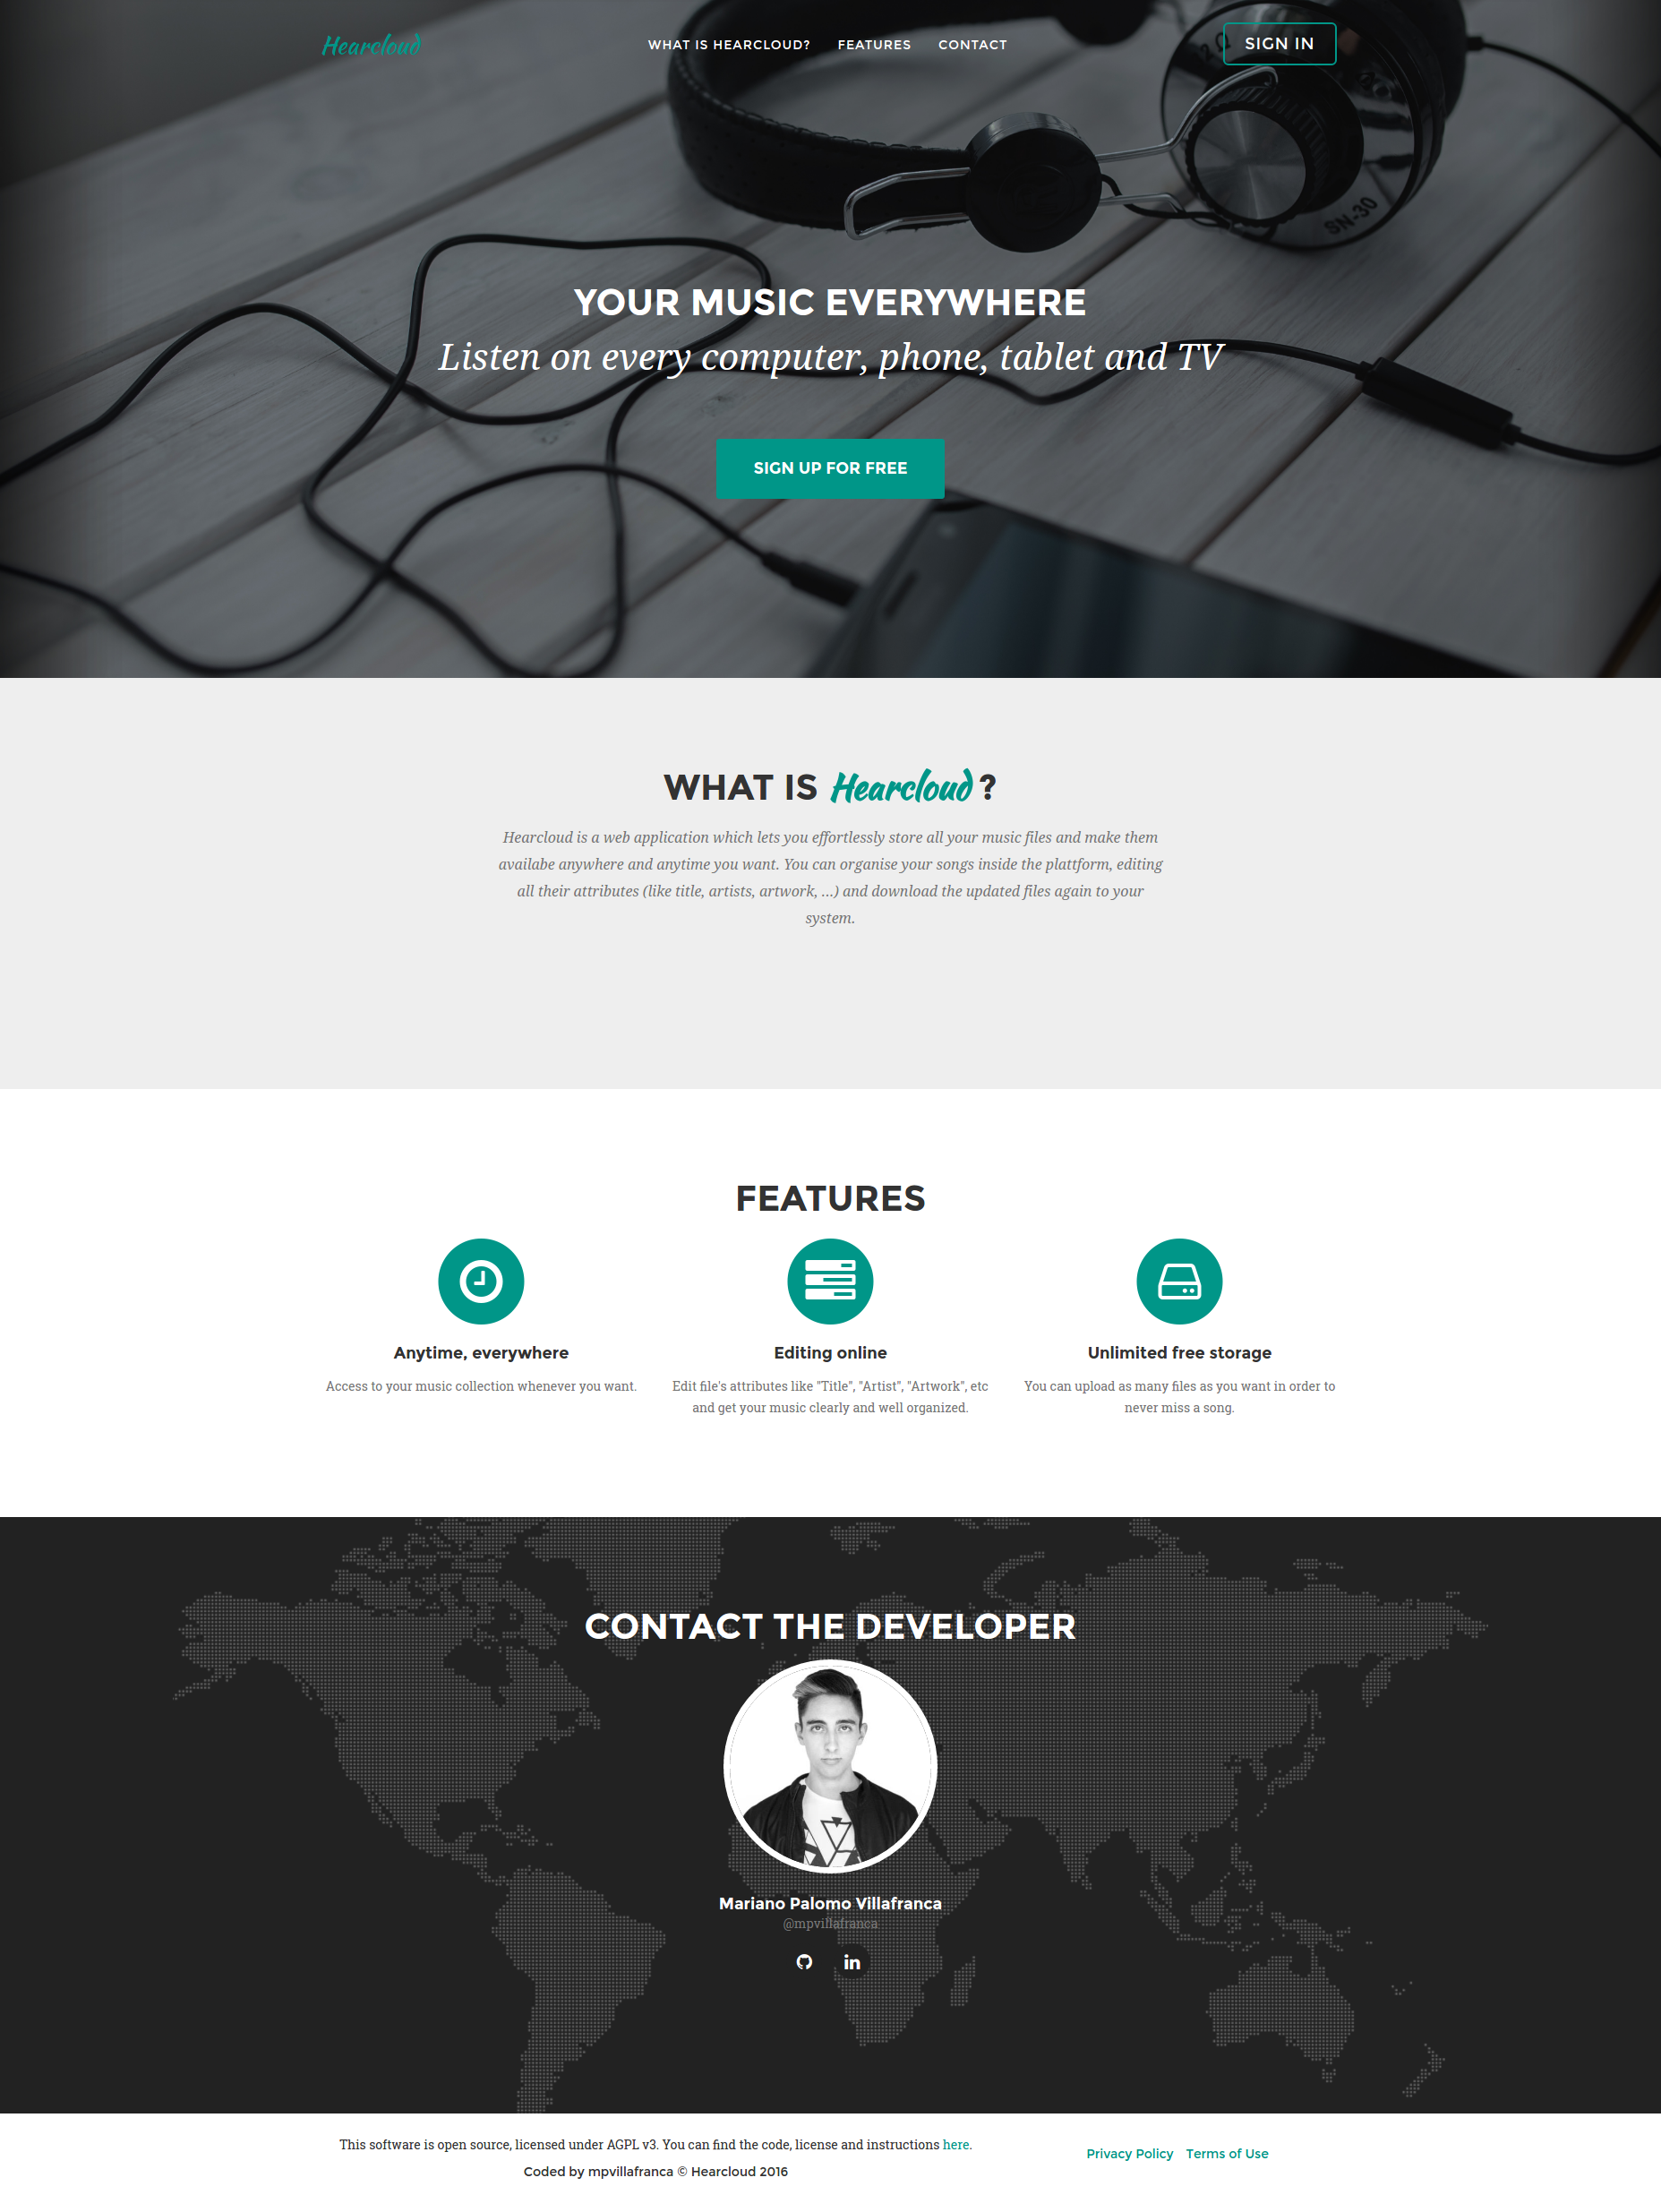
\includegraphics[scale=0.2]{../images/um/um_1.png}
\caption{Página principal (usuario no autenticado)}
\end{figure}

\subsection{Registro y acceso al sistema de usuarios}

La página de registro consiste en un formulario en el que se le solicita al usuario que introduzca un nombre de usuario, un email y una contraseña. Además, se le da la opción de cancelar el registro (lo que le redireccionaría de vuelta a la página principal) o de iniciar sesión (si ya estuviera registrado en el sistema).

\begin{figure}[H] 
\centering 
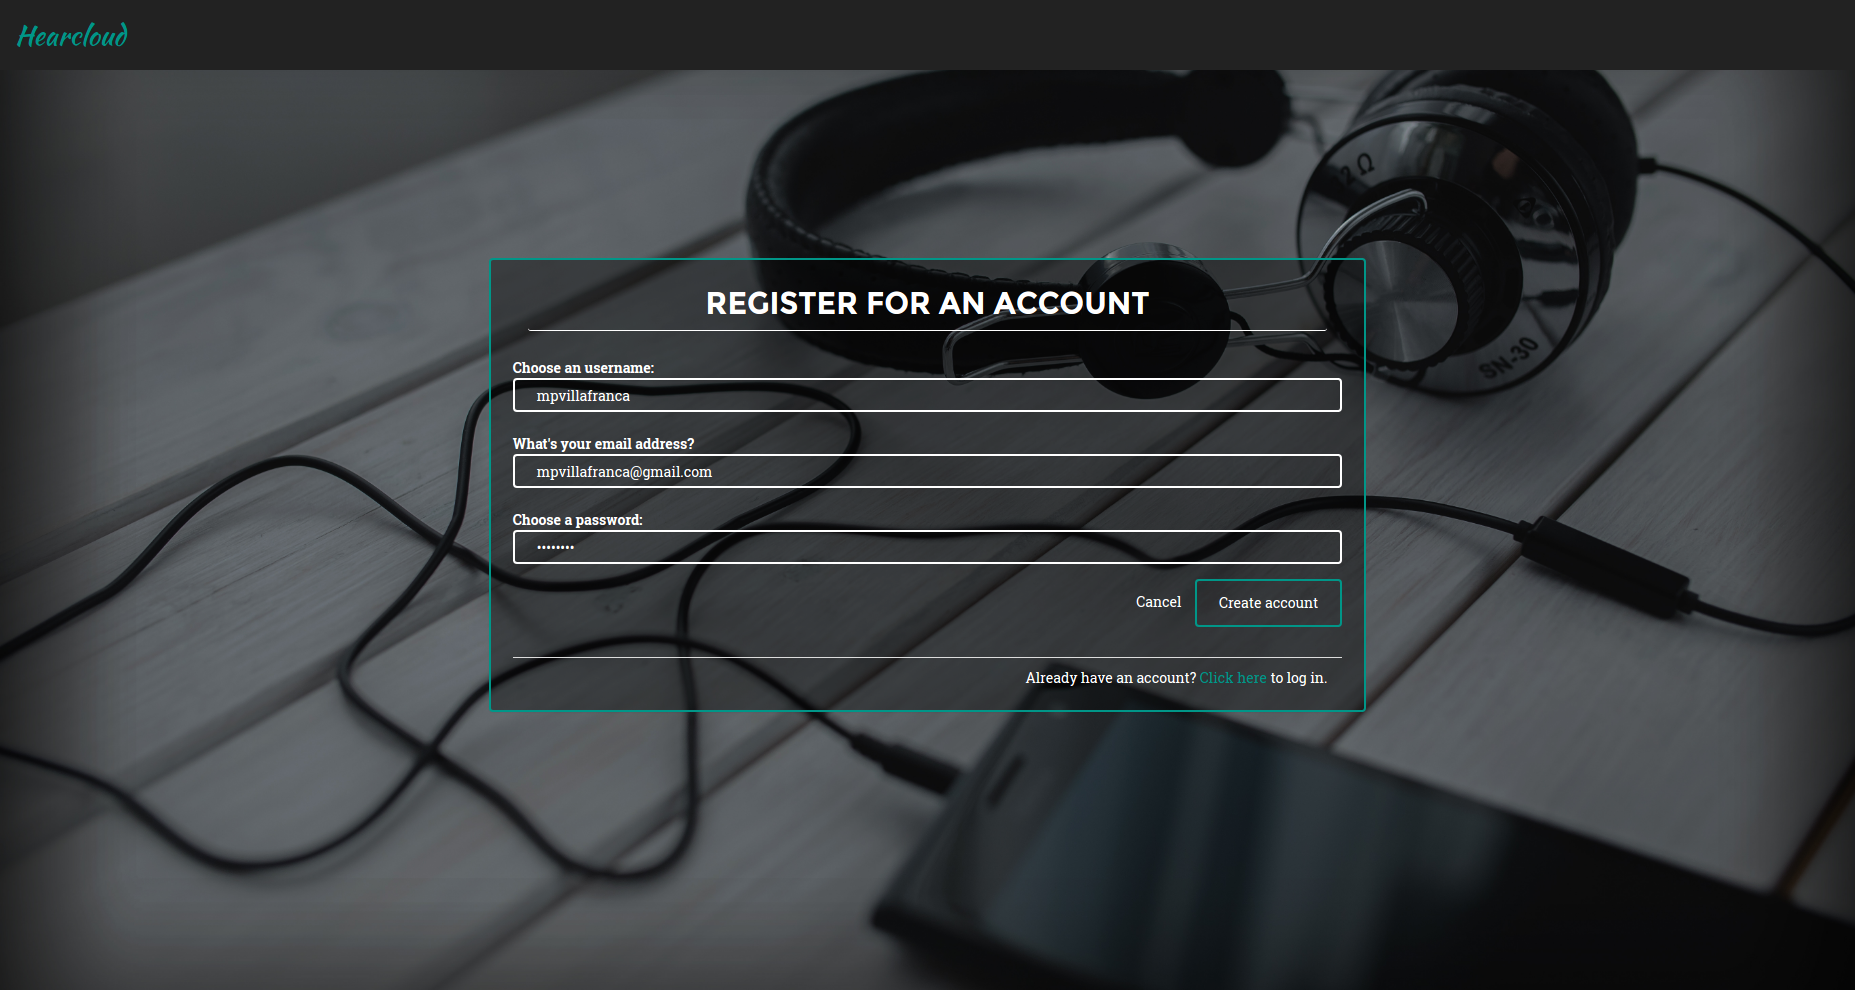
\includegraphics[scale=0.2]{../images/um/um_2.png}
\caption{Página de registro de usuarios}
\end{figure}

Al igual que en el caso anterior, la página de inicio de sesión, en la que se muestra un formulario para introducir nombre de usuario y contraseña, da la posibilidad de cancelar el inicio o de acceder al formulario de registro.

\begin{figure}[H] 
\centering 
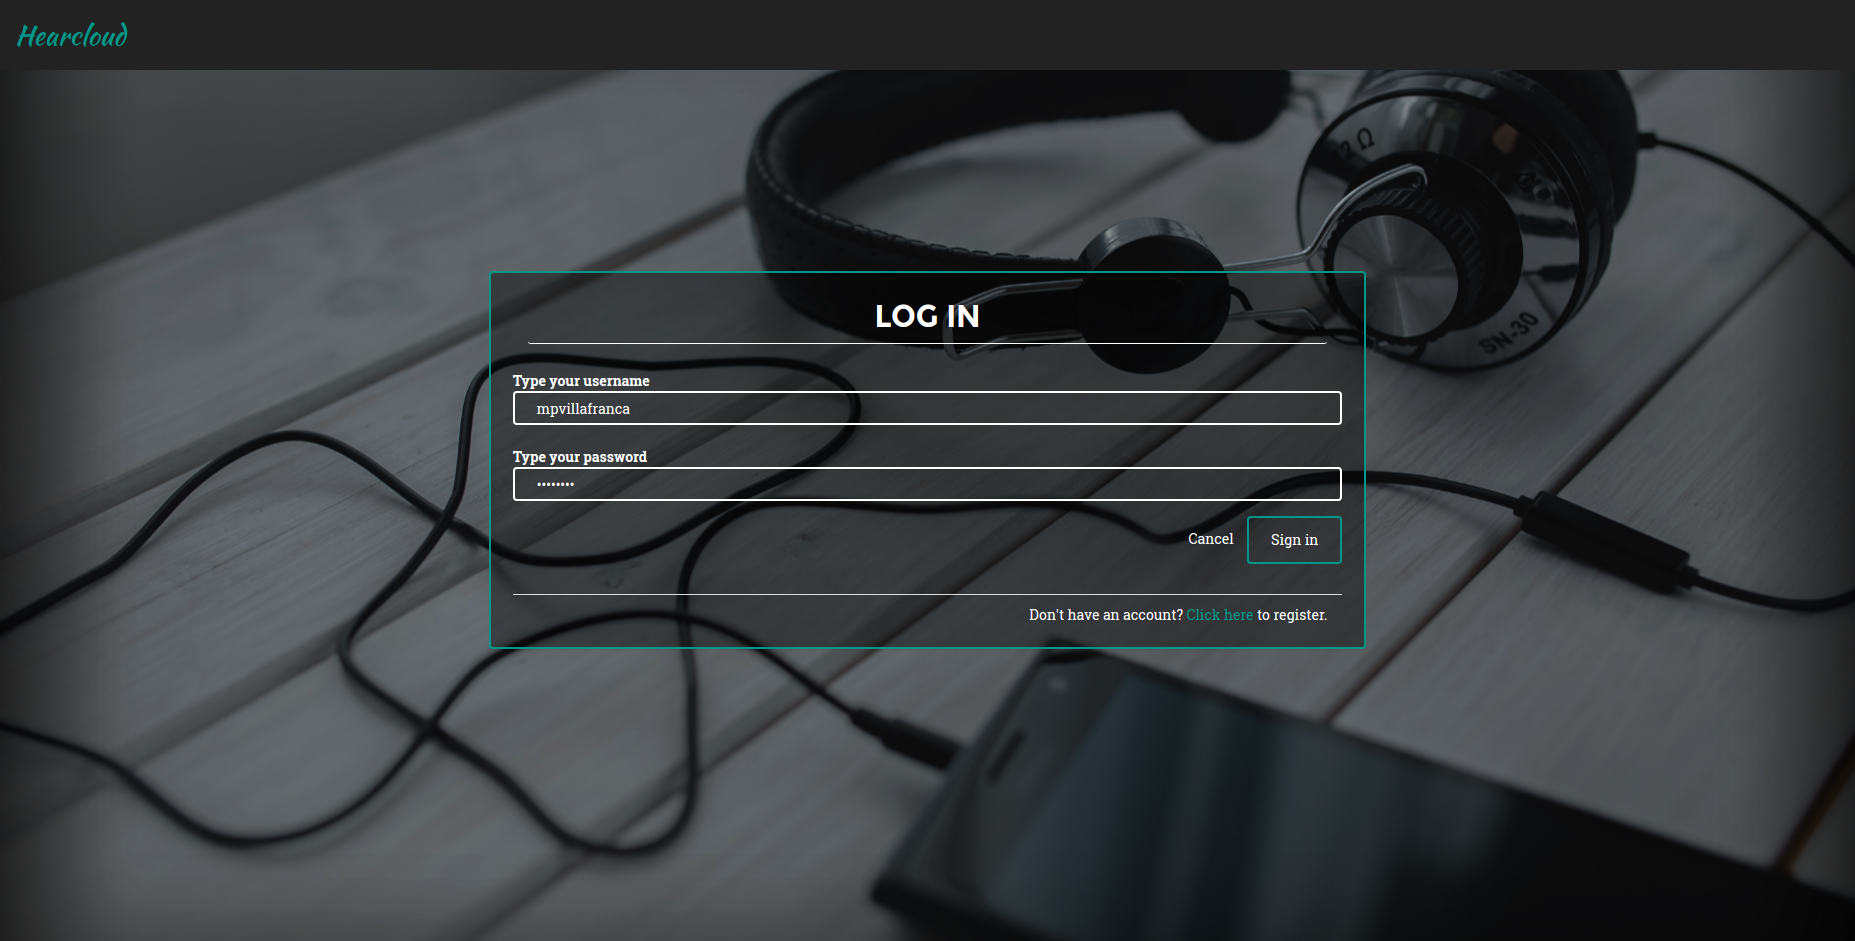
\includegraphics[scale=0.2]{../images/um/um_3.png}
\caption{Página de inicio de sesión de usuarios}
\end{figure}

\subsection{Panel principal del sistema: Canciones}

Es la vista principal del sistema para los usuarios que han iniciado sesión en la plataforma. Si es la primera vez que acceden, el panel central se mostrará vacío. Las canciones que el usuario vaya subiendo irán apareciendo en dicho panel, donde se muestra información básica acerca de la canción (imagen, título, artista, album, duración y fechas de subida y modificación). Por cada canción, aparecen tres acciones posibles a realizar en forma de botones: reproducir, descargar y eliminar.

Si se hace click en el botón de reproducir, se abrirá el reproductor integrado dentro del sistema, donde se muestran título y artista de la canción, junto a su portada y forma de onda. Además, nos podremos desplazar a lo largo de la canción para adelantarla o atrasarla. Se proporciona, por último, un boton que permite pausar la reproducción y reanudarla de nuevo en el punto en que se quedó.

Por otra parte, se ofrece la posibilidad al usuario de descargar el fichero de audio de vuelta a su sistema local, dándole la opción de realizar una conversión a otro formato de audio. Si la canción ha sido subida en un formato sin compresión (wav o aiff), las opciones de descarga serán cualquiera de los cuatro formatos disponibles (wav, aiff, m4a y mp3). Si la canción se subió en un formato con compresión (m4a y mp3), solo se podrán realizar conversiones entre dichos formatos.

\begin{figure}[H] 
\centering 
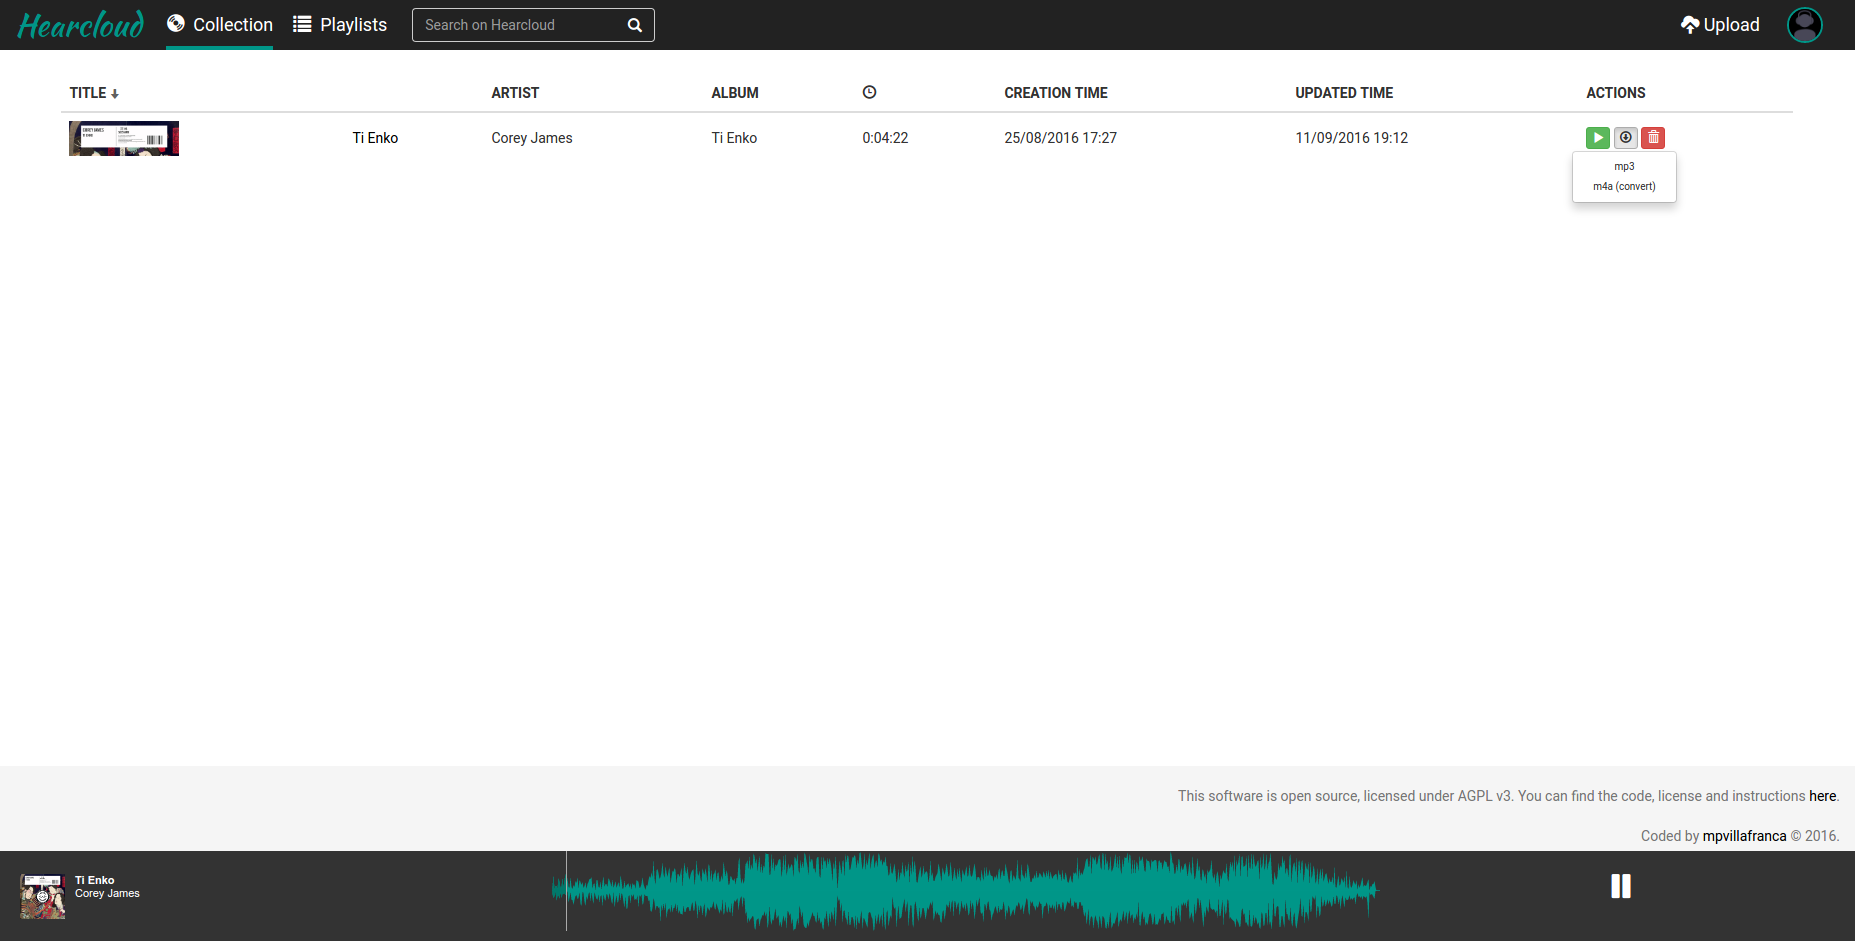
\includegraphics[scale=0.2]{../images/um/um_4.png}
\caption{Página principal (usuario autenticado)}
\end{figure}

Además, el usuario puede acceder a los detalles de la canción haciendo click en ella. En esta nueva ventana, se muestran todos los metadatos de la canción y se ofrece la posibilidad de editarlos mediante el correspondiente botón. Además, se vuelven a mostrar las opciones de reproducción, descarga y eliminación anteriores, cuyo comportamiento es idéntico al descrito anteriormente.

\begin{figure}[H] 
\centering 
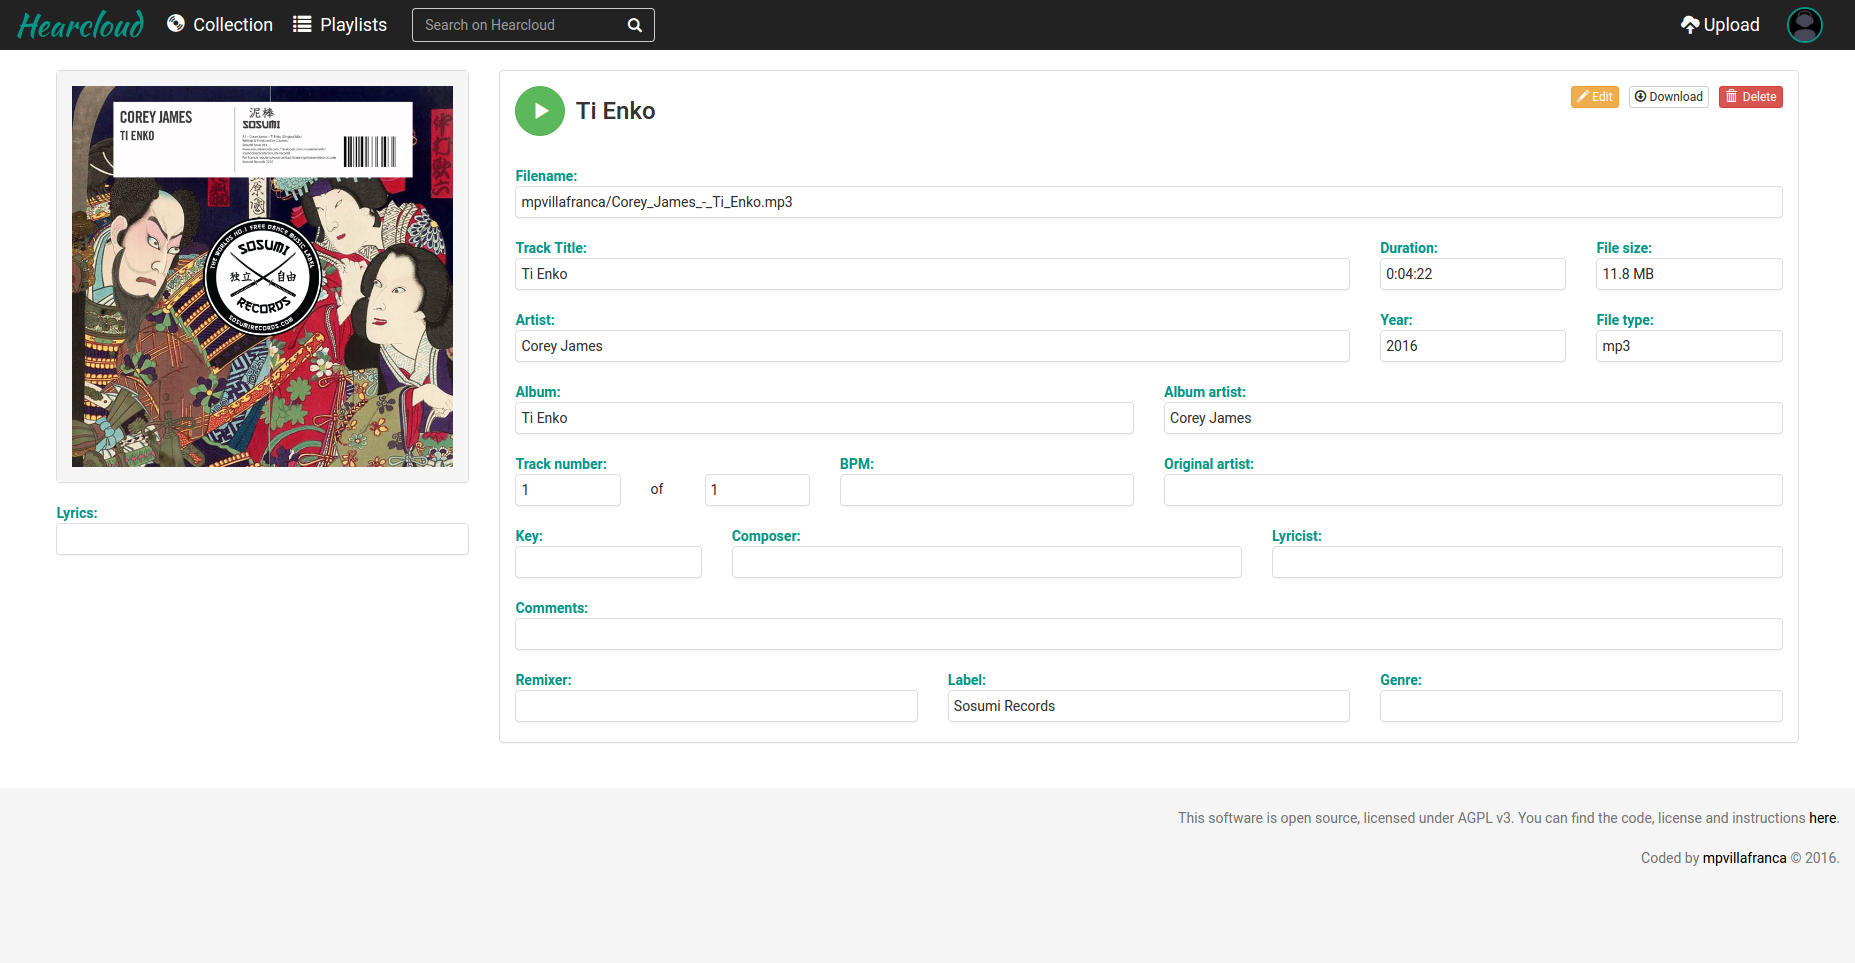
\includegraphics[scale=0.2]{../images/um/um_5.png}
\caption{Página del detalle de una canción}
\end{figure}

\subsection{Subida de ficheros}

Esta página es accesible mediante el botón \textit{Upload} situado en la barra de navegación del sistema. En ella, se da la posibilidad al usuario de subir a la plataforma cuantas canciones desee en una sola vez, aunque también puede seleccionar subir únicamente determinadas canciones de todas las seleccionadas inicialmente. Además, se ha implementado una \textit{drop zone}, donde el usuario puede arrastrar las canciones directamente desde el sistema sin necesidad de pulsar sobre el botón \texttt{Add files}.

\begin{figure}[H] 
\centering 
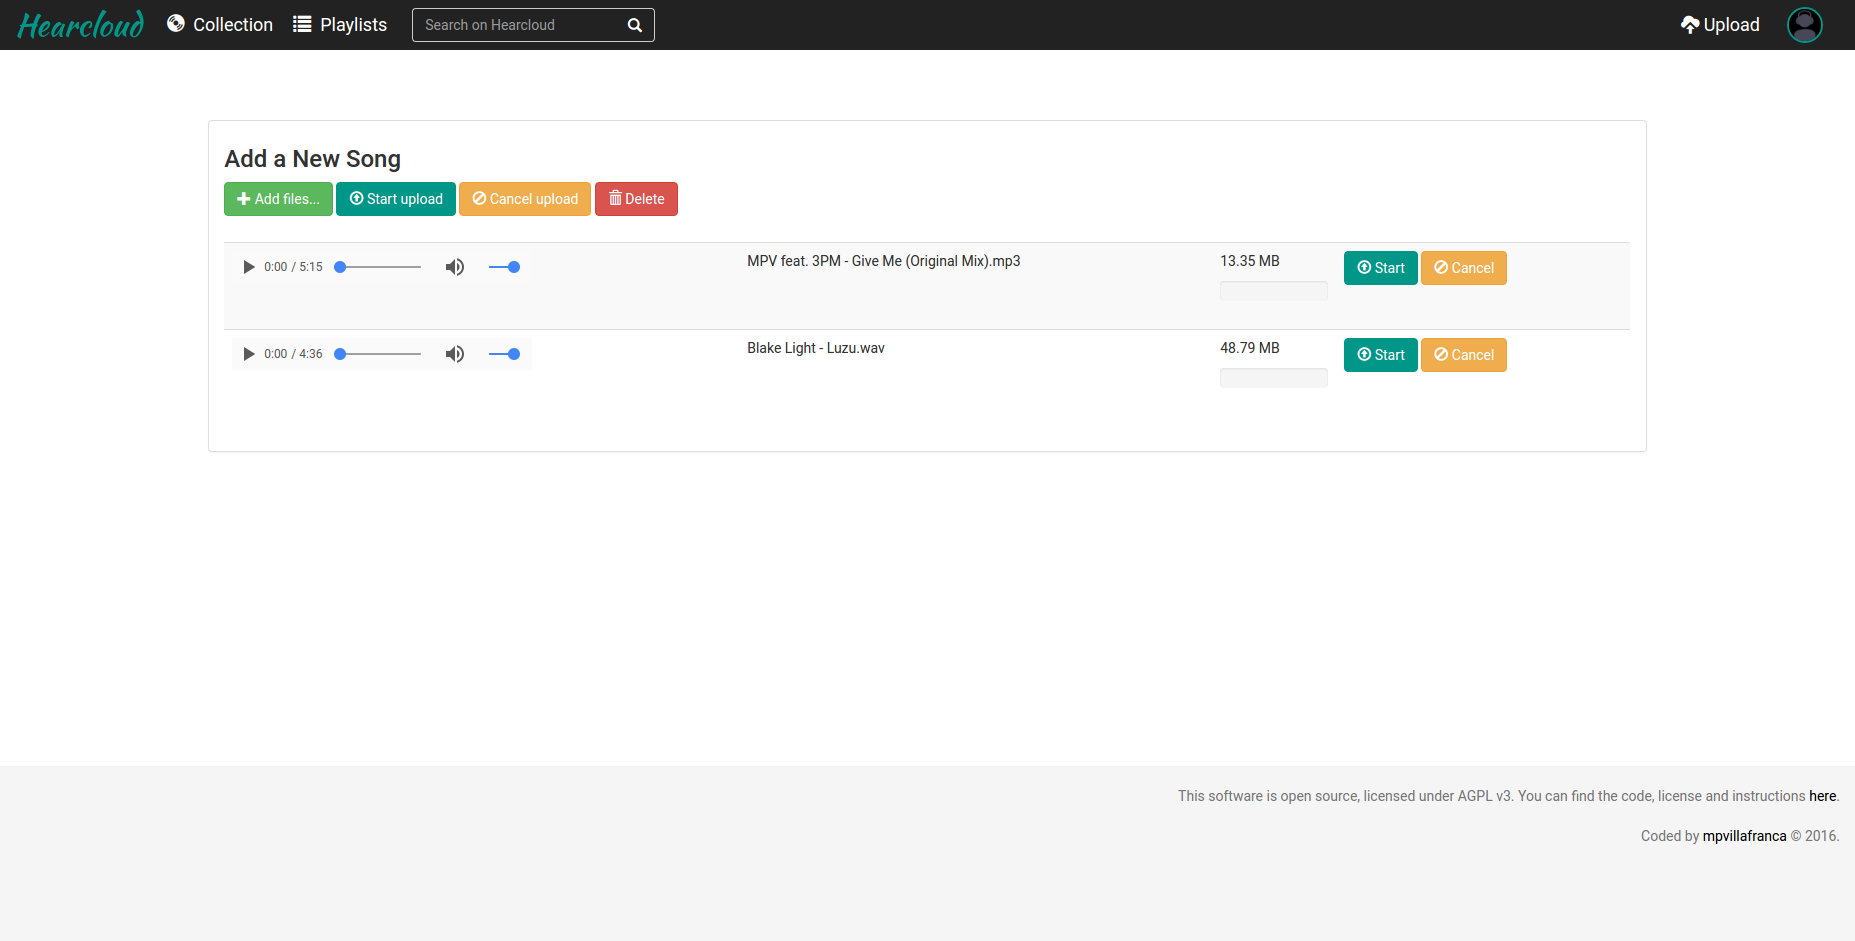
\includegraphics[scale=0.2]{../images/um/um_6.png}
\caption{Página de subida de canciones}
\end{figure}

\subsection{Panel perfil de usuario}

Este panel es accesible a través de la imagen de perfil del usuario situada en el borde superior derecho de la barra de navegación. En ella, se muestra la imagen de perfil del usuario, sus datos básicos y un contador sobre el número de canciones y listas de reproducción que tiene en su sistema.

\begin{figure}[H] 
\centering 
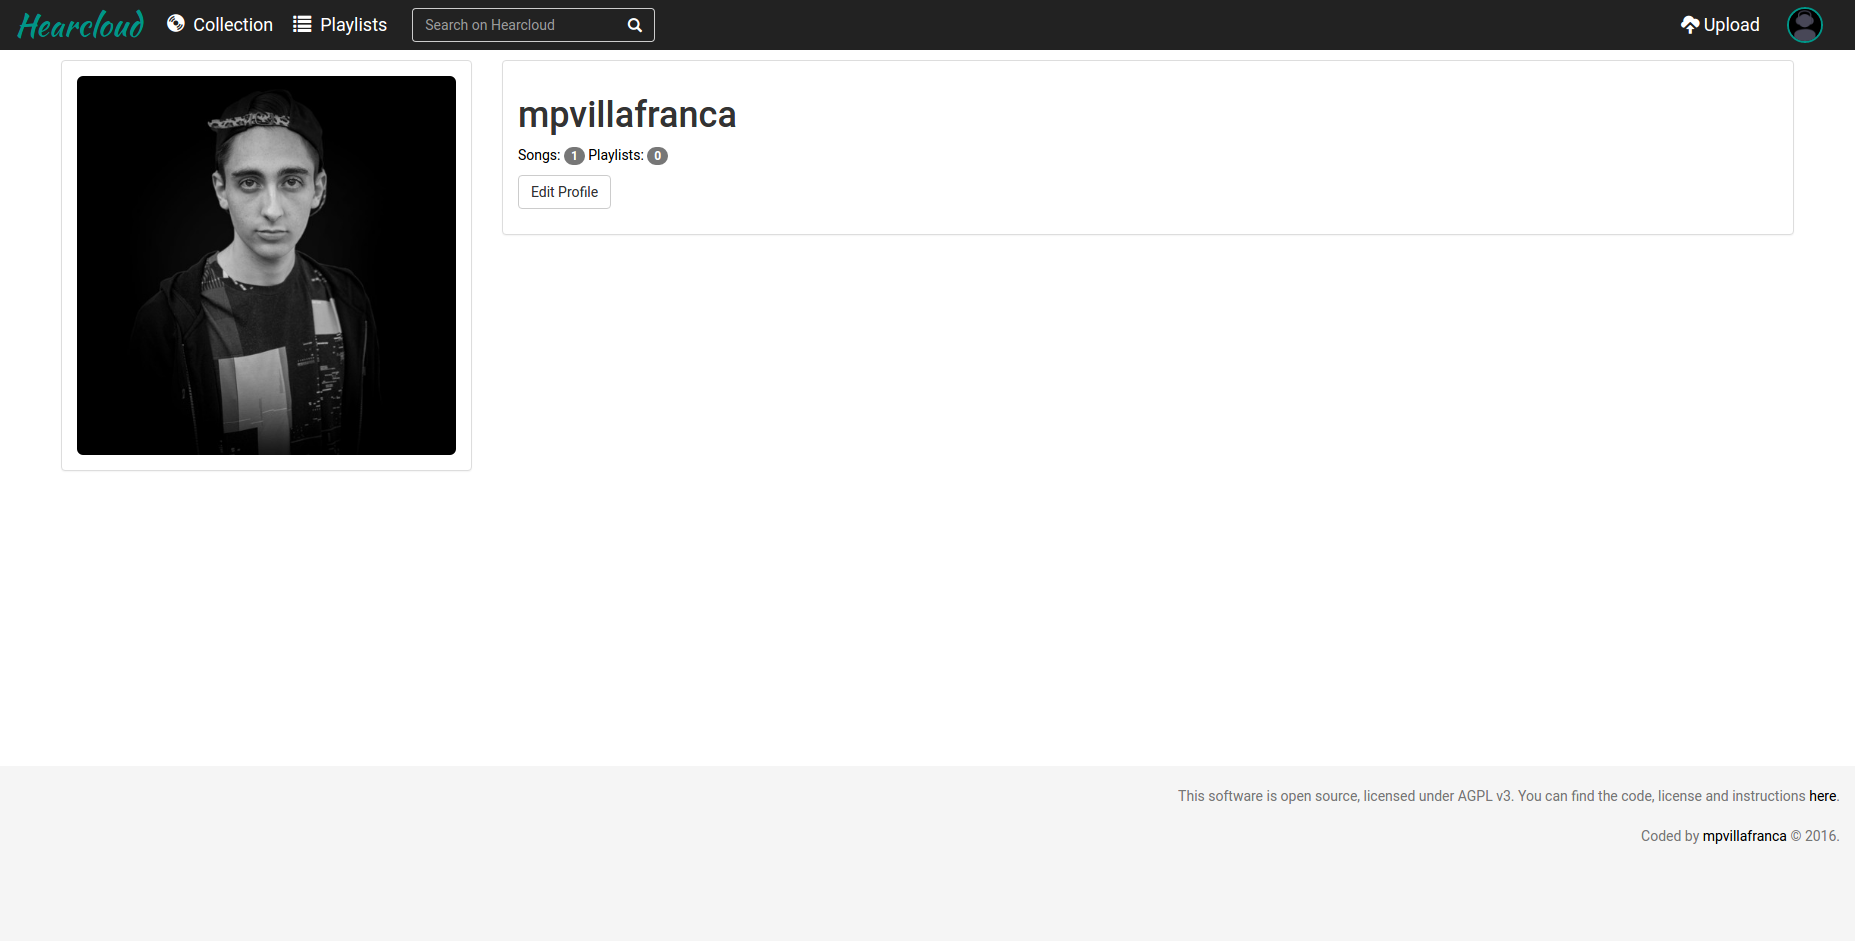
\includegraphics[scale=0.2]{../images/um/um_7.png}
\caption{Página del perfil de usuario}
\end{figure}

\subsection{Panel de administración}

Django ofrece un panel de administración accesible a través de la url \texttt{/admin}, al que podrán acceder todos los usuarios que tengan activado el atributo \texttt{is\_staff}. Las opciones que aquí se les muestren dependerán de los permisos que se les concedan. 

\begin{figure}[H] 
\centering 
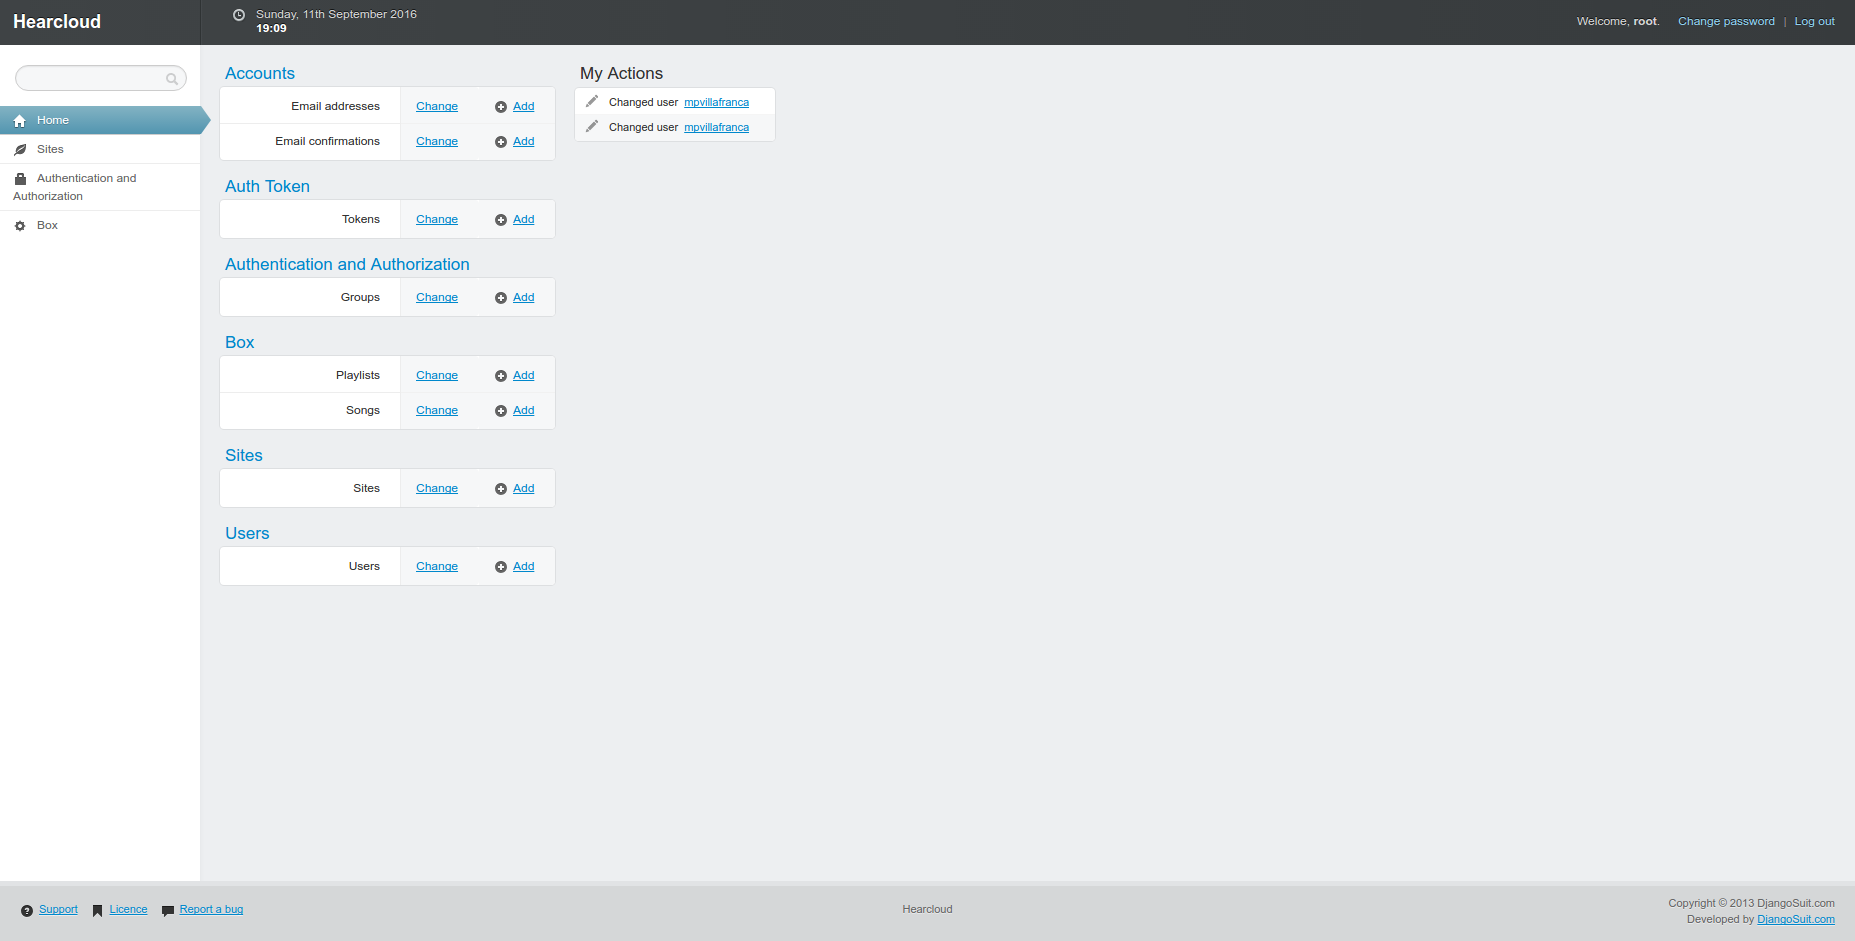
\includegraphics[scale=0.2]{../images/um/um_8.png}
\caption{Panel de administración de Django. Vista principal.}
\end{figure}

Si el usuario que accede posee todos los permisos o es superusuario, se desplegarán todas las opciones disponibles. Con él, podremos gestionar los usuarios y grupos del sistema y los ficheros y listas de reproducción que éstos almacenen.

\begin{figure}[H] 
\centering 
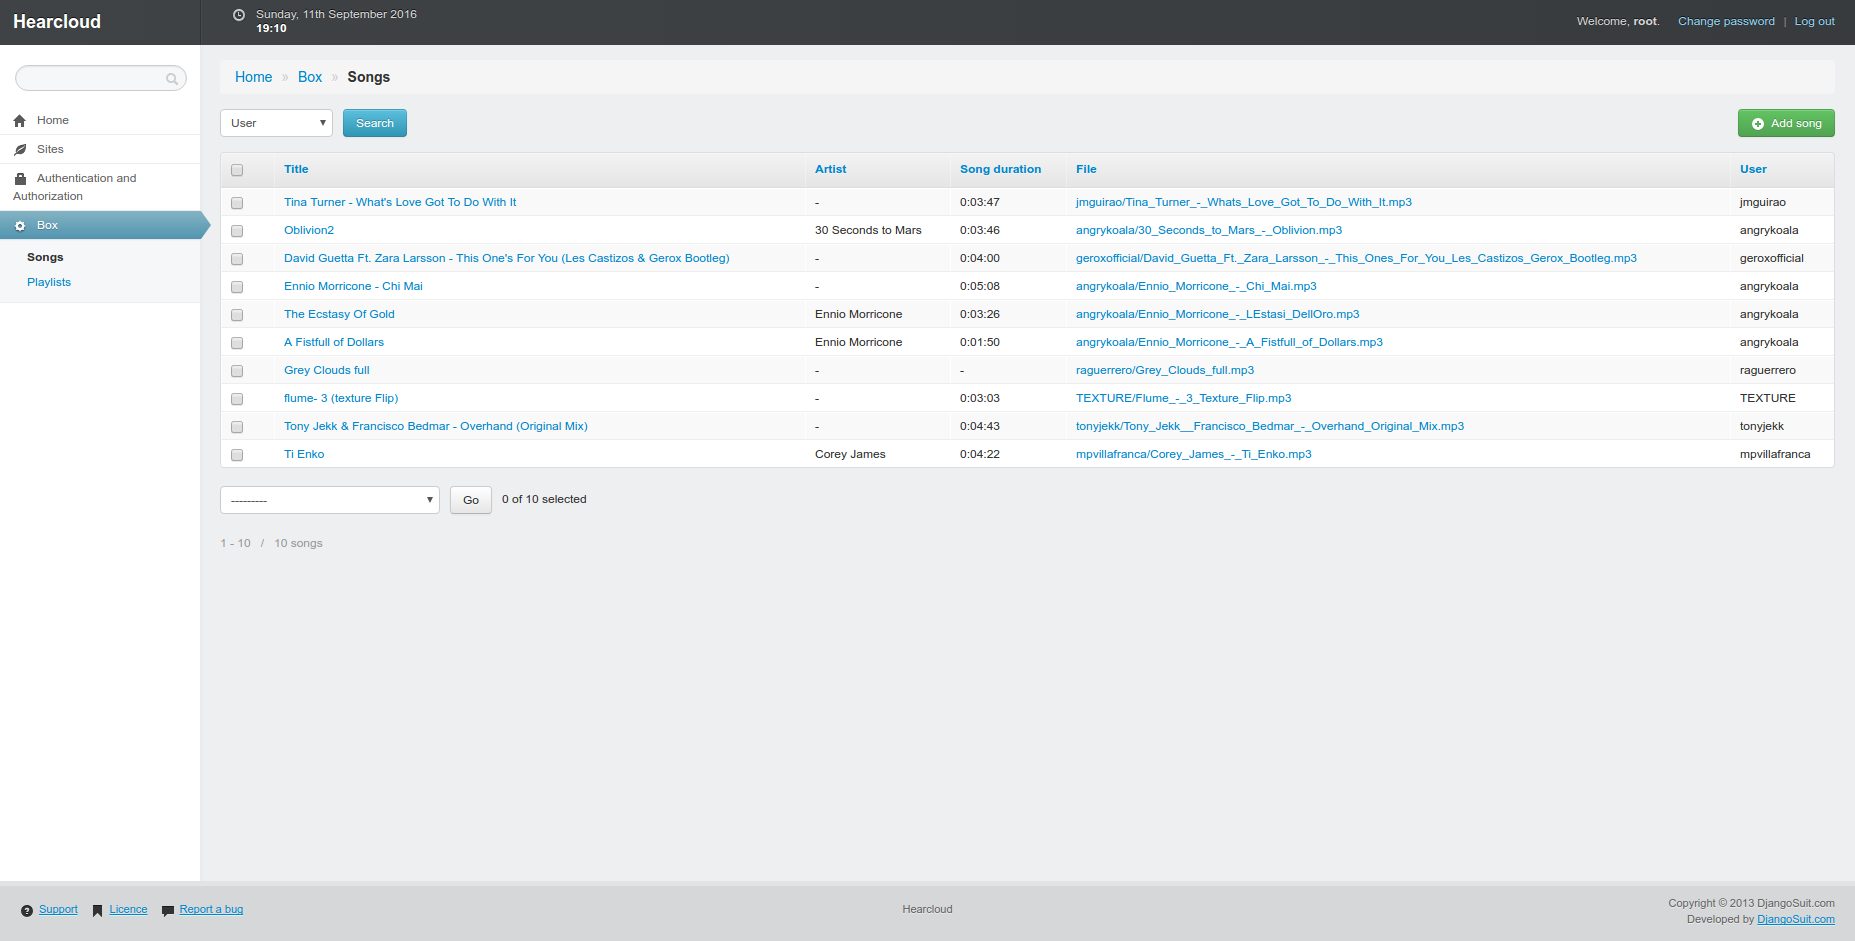
\includegraphics[scale=0.2]{../images/um/um_9.png}
\caption{Panel de administración de Django. Lista de canciones del sistema.}
\end{figure}

\subsection{Diseño adaptativo. Versión móvil}

Durante el desarrollo del sistema se ha tenido en cuenta que la plataforma se adapte lo máximo posible a los diferentes dispositivos desde los que se pueda acceder a ella, por lo que todas las secciones descritas anteriormente, deberían de visualizarse correctamente sin importar desde dónde se esté accediendo.

\begin{figure}[H]
\minipage{0.32\textwidth}
  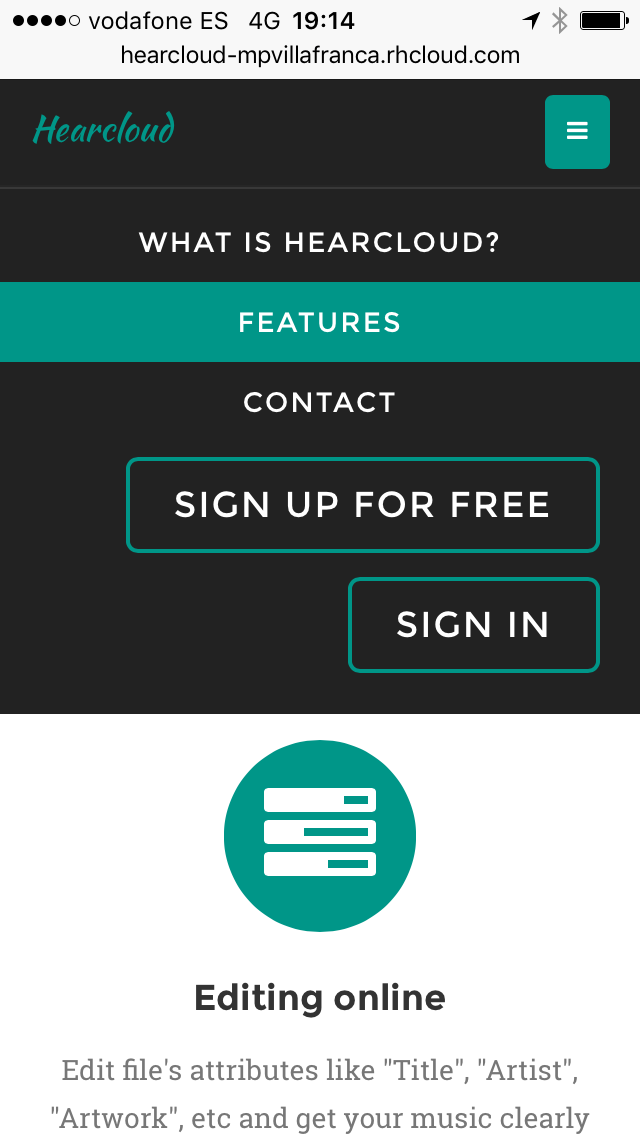
\includegraphics[width=\linewidth]{../images/um/um_10.png}
  \caption{Página principal (usuario no autenticado) en iPhone 6S}
\endminipage\hfill
\minipage{0.32\textwidth}
  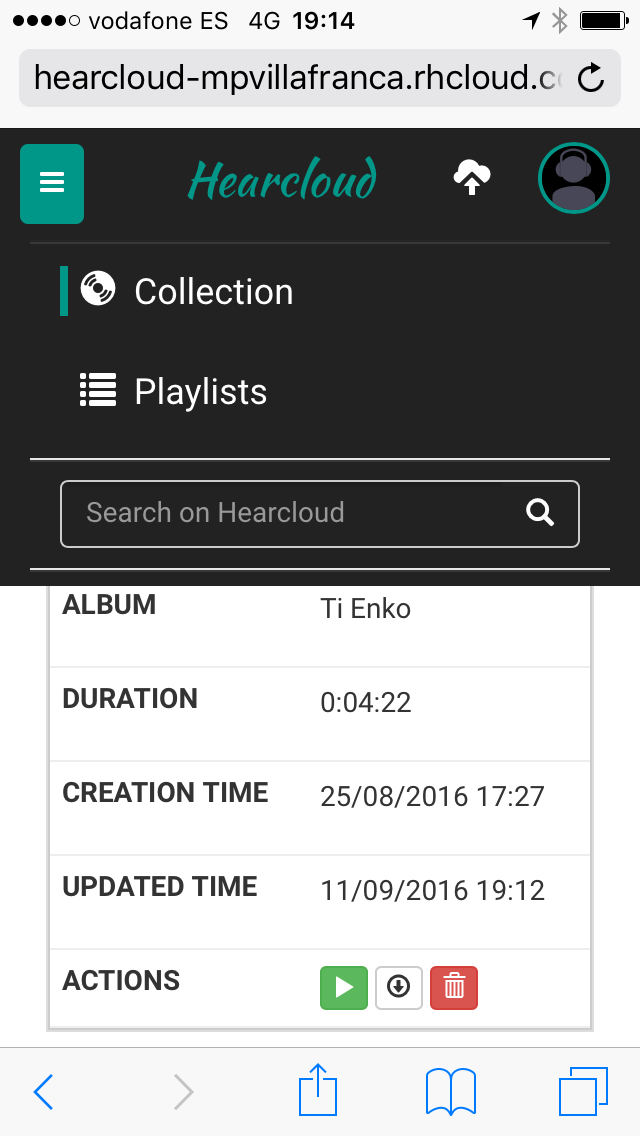
\includegraphics[width=\linewidth]{../images/um/um_11.png}
  \caption{Página principal (usuario autenticado) en iPhone 6S}
\endminipage\hfill
\end{figure}

\newpage

\section{Glosario de términos}
\label{sec:glosario}

\begin{sortedlist}
    \sortitem{\textbf{Frontend}: es la interfaz de la aplicación, es la parte de la aplicación que el usuario utiliza para comunicarse con la misma.}

    \sortitem{\textbf{Backend}: es el motor de una aplicación, se encarga de realizar las funciones en segundo plano que se encargan de que la aplicación funcione.}

    \sortitem{\textbf{Cloud}: }

    \sortitem{\textbf{Metadatos}: }

    \sortitem{\textbf{Software libre}: }

    \sortitem{\textbf{Framework}: }

    \sortitem{\textbf{Template}: }

    \sortitem{\textbf{Forja}: }

    \sortitem{\textbf{Streaming}: }

\end{sortedlist}

\newpage


\begin{thebibliography}{99}
	\addcontentsline{toc}{chapter}{Bibliografía}
\label{cap:bibliografia}

% ********************************************************************
% Bibliografía general
% ********************************************************************
\subsubsection*{Articulos y referencias generales consultados durante el desarrollo proyecto:}

% Comparación de tags entre diferentes formatos
\bibitem{TMMT} Tag Mapping - Mapping Tables \url{http://wiki.hydrogenaud.io/index.php?title=Tag_Mapping}

% Audio file metadata
\bibitem{PUMID3H} Python Useful Modules. ID3 Handling \url{https://wiki.python.org/moin/UsefulModules#ID3_Handling}

% Formularios con Ajax
\bibitem{DaAFS} Django and AJAX Form Submissions - Say ``Goodbye'' to the Page Refresh \url{https://realpython.com/blog/python/django-and-ajax-form-submissions/}


A continuación se presenta la bibliografía consultada en cada uno de los apartados de este proyecto.

\bigskip

% ********************************************************************
% Introducción
% ********************************************************************
\subsubsection*{Introducción.}

\bibitem{HDRDS} Historia del registro del sonido. \url{https://es.wikipedia.org/wiki/Historia_del_registro_del_sonido}

% ********************************************************************
% Objetivos
% ********************************************************************
\subsubsection*{Objetivos.}

% ********************************************************************
% Planificación y Analisis
% ********************************************************************
\subsubsection*{Planificación y análisis.}

\bibitem{Spotify} Spotify. \url{https://www.spotify.com/}

\bibitem{WikiSpotify} Wikipedia: Spotify. \url{https://en.wikipedia.org/wiki/Spotify}

\bibitem{SCYUYOM} Spotify: Can you upload your own music? \url{https://community.spotify.com/t5/Desktop-Linux-Windows-Web-Player/Can-you-upload-your-own-music/m-p/41511}

\bibitem{VLPPPSP} Spotify: ¿Vale la pena pagar por spotify premium? \url{http://curiotek.com/2015/03/01/vale-la-pena-pagar-por-spotify-premium/}

\bibitem{Soundcloud} Soundcloud. \url{https://soundcloud.com}

\bibitem{WikiSoundcloud} Wikipedia: Soundcloud. \url{https://en.wikipedia.org/wiki/SoundCloud}

\bibitem{ACP} Amazon Cloud Player. \url{https://music.amazon.com}

\bibitem{AUMIYML} Amazon Music. Help \& Customer Service. \url{https://www.amazon.com/gp/help/customer/display.html/ref=hp_bc_nav?ie=UTF8&nodeId=201377280}

\bibitem{GPM} Google Play Music. \url{https://www.play.google.com/music}

\bibitem{WikiGPM} Wikipedia: Google Play Music. \url{https://es.wikipedia.org/wiki/Google_Play_Music}

\bibitem{MMC} My Music Cloud. \url{https://www.mymusiccloud.com}

\bibitem{FAQMMC} My Music Cloud. Preguntas frecuentes. \url{http://support.mymusiccloud.com/}

\bibitem{GMELNEL} ``Guardar música en la nube es legal''. Laia Reventós, 24/08/2011. \url{http://elpais.com/diario/2011/08/24/radiotv/1314136802_850215.html}

% ********************************************************************
% Diseño
% ********************************************************************
\subsubsection*{Diseño.}

% ********************************************************************
% Implementación
% ********************************************************************
\subsubsection*{Implementación.}

% ********************************************************************
% Pruebas
% ********************************************************************
\subsubsection*{Pruebas.}

% ********************************************************************
% Pruebas
% ********************************************************************
\subsubsection*{Conclusiones.}

% ********************************************************************
% APIs
% ********************************************************************
\subsubsection*{Páginas de consulta sobre licencias y APIs del software utilizado:}
\bibitem{CC} Creative Commons. \url{http://creativecommons.org/licenses/}
\bibitem{Dj} Django. \url{https://www.djangoproject.com/}
\bibitem{J2} Jinja2. \url{https://www.djangoproject.com/}

\bibitem{TCI} {\tt Travis CI}. \url{http://docs.travis-ci.com/}

\bigskip


% ********************************************************************
% Otro material
% ********************************************************************
\subsubsection*{Otro material}
\begin{itemize}
	\item Diversas consultas puntuales al sitio {\tt Stack OverFlow}.
	\item Material docente de las asignaturas \textbf{Fundamentos de Ingeniería del Software}, \textbf{Desarrollo de Aplicaciones para Internet} e \textbf{Infraestructura Virtual} impartidas en el \textbf{Grado en Ingeniería Informática} en la \textbf{Universidad de Granada}.
\end{itemize}

\end{thebibliography}


\thispagestyle{empty}
\end{document}
